\documentclass[11pt]{article}
\usepackage[a4paper,margin=1in]{geometry}
\usepackage{cmap}
\usepackage[T1]{fontenc}
\usepackage{lmodern}
\usepackage{amsmath,amssymb,amsthm}
\usepackage{booktabs,tabularx,tikz}
\usepackage{listings}
\usetikzlibrary{arrows.meta,positioning,shapes.geometric}
\definecolor{fundgeometry}{HTML}{236BA6}
\definecolor{fundanalysis}{HTML}{207C61}
\definecolor{fundlearning}{HTML}{CB7623}
\usepackage[numbers,sort&compress]{natbib}
\usepackage[hidelinks]{hyperref}
\lstset{basicstyle=\ttfamily\scriptsize,breaklines=true,columns=fullflexible,
  keepspaces=true,showstringspaces=false,frame=single,xleftmargin=1em,
  xrightmargin=1em}
\newtheorem{theorem}{Theorem}[section]
\newtheorem{proposition}[theorem]{Proposition}
\theoremstyle{definition}
\newtheorem{assumption}[theorem]{Assumption}
\newtheorem{example}{Example}[section]
\newcommand{\E}{\mathcal E}
\newcommand{\pr}{\operatorname{pr}}
\title{Lie Symmetry Reduction for Parameter-Dependent PDEs:\\
Local Verification and Semi-Analytical Neural Approximation}
\author{}
\date{}
\begin{document}
\maketitle
\begin{abstract}
We organize local Lie-symmetry reduction of parameter-dependent nonlinear
partial differential equations as an explicit mathematical verification
contract. Standard point-symmetry, Frobenius and invariant-section results
are stated with hypotheses, local proofs and attribution. The construction
separates equation symmetry from graph invariance, gives the full coordinate
map and derivative pullback, and retains data, branch and residual-measure
conditions. A published scalar shallow-water-inspired equation is used only
after the general core, to verify an exceptional-exponent reduction and audit
its physical interpretation. We specify a controlled experiment comparing
an additional equation-derived analytical prior with a reduced hard-data
PINN and a direct PDE PINN. Historical numerical reports are isolated from
this prospective protocol because their matching source and raw evidence
are not all recovered. New maximal classification, a uniform neural error
certificate, and a physical full-system SVE derivation are not claimed.
\end{abstract}

\section{Introduction}
A Lie point symmetry is a local transformation of independent and dependent
variables whose prolongation preserves the differential equation manifold.
It maps solutions to solutions. Selecting a subgroup and requiring a
particular solution graph to be invariant is an additional restriction:
it can remove orbit directions from the unknown profile while retaining
the original nonlinear derivative problem.

This paper asks when that restriction gives a PDE, an ODE or consistency
conditions; why symmetry dimensions and parameter strata differ; how
coordinates, data and norms transform; and which measured aspects of a
reduction can inform a subsequent learning problem. A useful verified
subgroup is sufficient for a local invariant-family reduction. A claim
about the maximal point algebra requires a stronger classification proof.

The mathematical core is independent of the motivating PDE and credits
standard theory \cite{olver,anderson2000}. Section~\ref{sec:examples}
then provides worked examples and an audit of a published scalar benchmark
\cite{ap}. The ML contribution remains a bounded, testable protocol until
the numerical evidence gates in Section~\ref{sec:next-experiment} are met.
We separate fixed model parameters $\lambda$, data parameters $a$, group
parameters $\varepsilon$ and model perturbations $\delta$ throughout the
new development. The appendix preserves historical records with their
explicit evidence limitations.

\clearpage
\section{General reduction core and local proofs}
\label{sec:general-core}
\subsection{Decomposed fundamentals and unified notation}
\label{sec:decomposed-fundamentals}
The statements in this section are local, classical Lie-reduction results,
organized as a verification contract. Their foundations are the point-symmetry
and prolongation theory of \citet{olver} and the invariant-section and dynamic
reduction framework of \citet{anderson2000}. They are not claimed as new
classification or existence theorems. Concrete equations appear only in
Section~\ref{sec:examples}.

\begin{center}\small
\renewcommand{\arraystretch}{1.13}
\begin{tabularx}{\linewidth}{@{}p{3.2cm}X@{}}
\toprule
Notation & Fixed meaning throughout the reduction core \\
\midrule
$p,q,r,n$ & Counts of independent variables, fields, equations, and original differential order; $r=q$ is not required. \\
$\pi:E\to M$ & Local field bundle; $x=(x^1,\ldots,x^p)$ are base coordinates, $u=(u^1,\ldots,u^q)$ are fibre coordinates. \\
$\sigma:M\to E$ & A physical field/section; $j^n\sigma$ is its derivative jet. The coordinate $u$ and a section are distinct objects. \\
$\lambda,a,\varepsilon,\delta$ & Fixed model parameters, data/integration parameters, group-flow displacement, and model perturbation, respectively. \\
$H,\mathfrak h,k,\ell$ & Selected local symmetry subgroup, its Lie algebra, $k=\dim\mathfrak h$, and base-orbit rank $\ell$. \\
$y,z,v,F$ & Orbit coordinates, quotient coordinates, invariant field coordinates, and the unknown reduced profile. \\
$\Delta,\mathcal R,\mathcal T$ & Original residual, reduced residual, and reconstruction map. \\
$J,\alpha,i,b$ & Derivative multi-index; field, base-coordinate and generator indices. Repeated applicable indices are summed. \\
\bottomrule
\end{tabularx}
\end{center}

At fixed $\lambda$, specify the problem as
\begin{equation}
 \mathcal P_\lambda=
 \bigl(\Omega,\Delta,\mathcal N,\mathcal A,
       \{(\Gamma_j,\mathcal B_j)\}_{j=1}^{N_B};\lambda\bigr),\qquad
 \mathcal E_\lambda=\{\Delta_A(x,u^{(n)};\lambda)=0\}_{A=1}^r\subset J^n(E).
 \label{eq:formal-problem}
\end{equation}
Here $\Omega\subset M$ is the domain, $\mathcal N$ records nonzero factors,
$\mathcal A$ records smoothness/sign/branch assumptions, and $\mathcal B_j=0$
is prescribed on the supplied data surface $\Gamma_j$. The derivative budget
also covers the data operators. Work on a regular equation chart or record
redundant equations and their rank explicitly. Smooth real branches and every
denominator remain part of the problem after symbolic simplification.

The ordinary finite-order jet construction below assumes integer differential
order and point transformations. Fractional/nonlocal operators require a
separate operator-action and chain-rule contract; they are not obtained by
replacing $n$ by a noninteger in the formulas.

\subsection{Point actions, prolongation and the infinitesimal criterion}
\label{sec:prolongation-core}
A local point action $\Phi_\varepsilon(x,u)=(\bar x,\bar u)$ acts on a field
when its transformed graph is still a graph. Its generator and characteristic are
\begin{equation}
 X=\xi^i(x,u;\lambda)\partial_{x^i}
       +\eta^\alpha(x,u;\lambda)\partial_{u^\alpha},\qquad
 Q^\alpha=\eta^\alpha-\xi^i u_i^\alpha.
 \label{eq:characteristic-core}
\end{equation}
The flow solves $d\bar x^i/d\varepsilon=\xi^i(\bar x,\bar u)$ and
$d\bar u^\alpha/d\varepsilon=\eta^\alpha(\bar x,\bar u)$, with the original
point as initial condition. Parameters $\lambda$ remain fixed. At fixed base
coordinates the infinitesimal field change is $Q[j^1\sigma]$.

Prolongation is the derivative chain rule, not an independently chosen symmetry.
With $u_0^\alpha=u^\alpha$ and $\eta_0^\alpha=\eta^\alpha$,
\begin{align}
 D_i&=\partial_{x^i}+\sum_{\alpha,J}u_{J+e_i}^\alpha\partial_{u_J^\alpha},\\
 \eta_{J+e_i}^\alpha&=D_i\eta_J^\alpha-u_{J+e_j}^\alpha D_i\xi^j,\\
 \pr^{(n)}X&=X+\sum_{\alpha,\,1\le |J|\le n}
                      \eta_J^\alpha\partial_{u_J^\alpha}.
 \label{eq:prolongation-core}
\end{align}
Total derivatives are understood on the infinite jet bundle, or with enough
higher jets for each finite calculation. The equivalent expression
$\eta_J^\alpha=D_JQ^\alpha+\xi^iu_{J+e_i}^\alpha$ has cancellation of the
apparent higher-order jets for a point generator.

\begin{proposition}[Local infinitesimal symmetry criterion]
\label{prop:infinitesimal-core}
Let $\mathcal E_\lambda$ be a smooth equation submanifold on a regular jet
chart, and let the prolonged local point flow be defined there. The flow
preserves $\mathcal E_\lambda$ locally if and only if
\begin{equation}
 \left.\pr^{(n)}X(\Delta_A)\right|_{\mathcal E_\lambda}=0
 \quad\text{for every defining equation }A.
 \label{eq:determining}
\end{equation}
When the defining residuals are independent, this is locally equivalent to
$\pr^{(n)}X(\Delta)=C_X\Delta$ for a smooth multiplier matrix $C_X$.
\end{proposition}
\begin{proof}
Preservation differentiates to tangency. Conversely, a smooth tangent vector
field has a local flow in the submanifold by uniqueness of its flow equations.
On a regular defining chart, a smooth function vanishing on the submanifold
is a smooth linear combination of its defining coordinates (Hadamard's lemma),
which gives the multiplier form. Redundant or singular equations require
their own defining chart; the rank hypothesis cannot be discarded.
\end{proof}

Equation symmetry and graph invariance are separate conditions:
\begin{equation}
 \underbrace{\pr^{(n)}X_b\Delta|_{\mathcal E_\lambda}=0}_{\text{maps solutions to solutions}},
 \qquad
 \underbrace{Q_b^\alpha[j^1\sigma]=0}_{\text{fixes this solution graph}}.
 \label{eq:fundamental-tangencies}
\end{equation}
An invariant quantity $I$ instead satisfies $X_bI=0$. Thus an orbit, a field
coordinate, an invariant quantity, and an invariant solution are not
interchangeable. Nonclassical symmetry tests tangency on the joint PDE and
invariant-surface system, including its differential consequences; it has a
different contract from classical point symmetry.

\subsection{Canonical coordinates and the local reconstruction theorem}
\label{sec:canonical-core}
Choose a finite-dimensional local subgroup $H$ of verified equation symmetries.
An infinite-dimensional full point algebra does not prevent this choice.

\begin{assumption}[Regular transverse local reduction]
\label{ass:reduction-core}
On a connected local chart, the action is projectable:
$X_b=\xi_b^i(x;\lambda)\partial_{x^i}+\eta_b^\alpha(x,u;\lambda)\partial_{u^\alpha}$.
Its selected fields close as a Lie subalgebra and have constant ranks
\begin{equation}
 \ell=\operatorname{rank}[\xi_b^i]
      =\operatorname{rank}[\xi_b^i,\eta_b^\alpha],\qquad 0\le\ell\le p.
 \label{eq:fundamental-rank}
\end{equation}
Take smooth base coordinates $(y,z)$, where $y\in\mathbb R^\ell$ and
$z\in\mathbb R^d$, $d=p-\ell$, and invariant fibre coordinates
$v=I(x,u)\in\mathbb R^q$ satisfying
\begin{equation}
 X_bz^a=0,\quad X_bI^\alpha=0,\quad
 \det D_x(y,z)\ne0,\quad \det I_u\ne0.
 \label{eq:canonical-checks}
\end{equation}
The resulting local quotient bundle is smooth. Restrict all flows to the
connected orbit segments in this chart; no global quotient is assumed.
\end{assumption}

\begin{theorem}[Local canonical form and invariant sections]
\label{thm:canonical-core}
Under Assumption~\ref{ass:reduction-core}, the coordinate map and its inverse are
\begin{equation}
 \chi:(x,u)\longmapsto(y(x),z(x),I(x,u)),\qquad
 x=\Theta(y,z),\quad u=\Psi(\Theta(y,z),v).
 \label{eq:reduction-chart}
\end{equation}
The orbit distribution becomes $\operatorname{span}\{\partial_{y^1},\ldots,
\partial_{y^\ell}\}$. The $H$-invariant local sections correspond bijectively
to reduced profiles through
\begin{equation}
 v=F(z),\qquad
 u=\mathcal T_{\lambda,H}F:=\Psi(x,F(z(x))).
 \label{eq:fundamental-reconstruction}
\end{equation}
\end{theorem}
\begin{proof}
Lie closure and constant rank make the orbit distribution involutive;
Frobenius' theorem gives adapted local coordinates. Projectability permits
the base coordinates to be chosen independently of $u$. Equal base and total
ranks make the infinitesimal isotropy act trivially in the fibre on this
local transverse chart. The invariant coordinates and nonzero Jacobians give
a local inverse by the inverse function theorem. In these coordinates,
$Q_b=0$ says that the section is constant in every orbit direction:
$\partial_yv=0$. Connectedness gives $v=F(z)$. Conversely, $v=F(z)$ has an
orbit-invariant graph, and the inverse chart reconstructs it uniquely.
\end{proof}

For a single nonvanishing generator, the flow-box theorem permits $Xy=1$.
For several noncommuting generators, Frobenius straightens their distribution,
not all generators simultaneously into commuting coordinate fields.
Solve the characteristic flow equations or the invariant PDEs $X_bI=0$;
ratios of characteristic differentials are usable only where their denominators
are nonzero. Explicitly check both inverse identities and the Jacobians.

\begin{center}
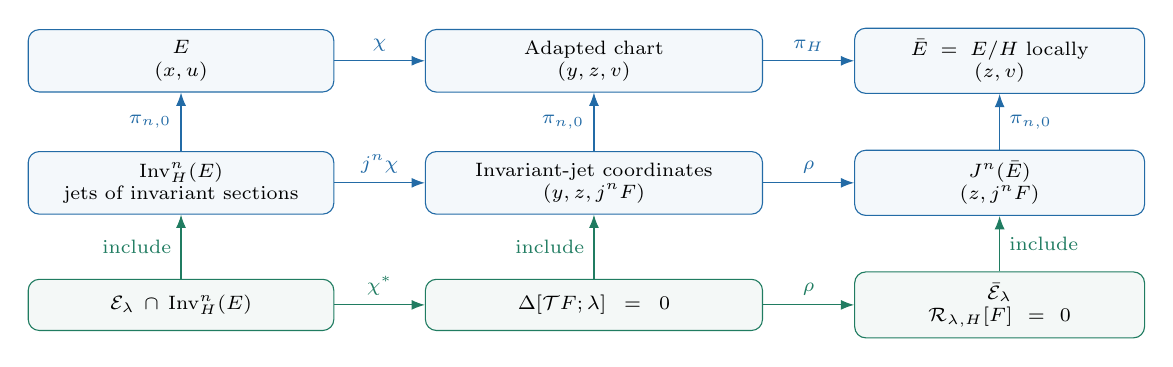
\begin{tikzpicture}[x=.92cm,y=1cm,>=Latex,
 every node/.style={font=\scriptsize},
 card/.style={draw=fundgeometry,fill=fundgeometry!5,rounded corners,
              align=center,inner sep=4pt,minimum height=.65cm}]
 \node[card,text width=3.6cm] (e) at (2.3,0) {$E$\\$(x,u)$};
 \node[card,text width=4.0cm] (c) at (8,0) {Adapted chart\\$(y,z,v)$};
 \node[card,text width=3.4cm] (q) at (13.6,0) {$\bar E=E/H$ locally\\$(z,v)$};
 \node[card,text width=3.6cm] (j) at (2.3,-1.55) {$\operatorname{Inv}_H^n(E)$\\jets of invariant sections};
 \node[card,text width=4.0cm] (jc) at (8,-1.55) {Invariant-jet coordinates\\$(y,z,j^nF)$};
 \node[card,text width=3.4cm] (jq) at (13.6,-1.55) {$J^n(\bar E)$\\$(z,j^nF)$};
 \node[card,draw=fundanalysis,fill=fundanalysis!5,text width=3.6cm] (s) at (2.3,-3.1)
  {$\mathcal E_\lambda\cap\operatorname{Inv}_H^n(E)$};
 \node[card,draw=fundanalysis,fill=fundanalysis!5,text width=4.0cm] (sc) at (8,-3.1)
  {$\Delta[\mathcal TF;\lambda]=0$};
 \node[card,draw=fundanalysis,fill=fundanalysis!5,text width=3.4cm] (sq) at (13.6,-3.1)
  {$\bar{\mathcal E}_\lambda$\\$\mathcal R_{\lambda,H}[F]=0$};
 \draw[->,fundgeometry] (e)--(c) node[midway,above] {$\chi$};
 \draw[->,fundgeometry] (c)--(q) node[midway,above] {$\pi_H$};
 \draw[->,fundgeometry] (j)--(jc) node[midway,above] {$j^n\chi$};
 \draw[->,fundgeometry] (jc)--(jq) node[midway,above] {$\rho$};
 \draw[->,fundanalysis] (s)--(sc) node[midway,above] {$\chi^*$};
 \draw[->,fundanalysis] (sc)--(sq) node[midway,above] {$\rho$};
 \draw[->,fundgeometry] (j)--(e) node[midway,left] {$\pi_{n,0}$};
 \draw[->,fundgeometry] (jc)--(c) node[midway,left] {$\pi_{n,0}$};
 \draw[->,fundgeometry] (jq)--(q) node[midway,right] {$\pi_{n,0}$};
 \draw[->,fundanalysis] (s)--(j) node[midway,left] {include};
 \draw[->,fundanalysis] (sc)--(jc) node[midway,left] {include};
 \draw[->,fundanalysis] (sq)--(jq) node[midway,right] {include};
\end{tikzpicture}
\par\smallskip\small
Coordinate adaptation, invariant jets, and equation reduction are separate,
compatible maps. Here $\pi_H$ forgets orbit coordinates, $j^n\chi$ is the
chain-rule jet map, and $\rho$ is the invariant-jet quotient. Prolongation
precedes restriction to invariant jets.
\end{center}

\begin{theorem}[Local reduced-equation and reconstruction equivalence]
\label{thm:reconstruction-core}
Assume the hypotheses above and that the invariant equation intersection and
its quotient have regular local defining charts. Then
\begin{equation}
 \bar{\mathcal E}_\lambda
   =\bigl(\mathcal E_\lambda\cap\operatorname{Inv}_H^n(E)\bigr)/H
       \subset J^n(\bar E).
 \label{eq:fundamental-pullback}
\end{equation}
For a $C^n$ profile $F$ whose reconstructed jet stays in the chart,
\begin{equation}
 \mathcal R_{\lambda,H}[F]=0
 \quad\Longleftrightarrow\quad
 \Delta[\mathcal T_{\lambda,H}F;\lambda]=0.
 \label{eq:reconstruction-equivalence}
\end{equation}
This correspondence is exactly between reduced solutions and invariant
original solutions on the stated chart. It need not preserve the original
number of independent defining residuals or their differential order.
\end{theorem}
\begin{proof}
Theorem~\ref{thm:canonical-core} identifies an invariant jet with
$(y,z,j^nF)$. The prolonged action preserves both the equation manifold and
invariant jets. Their intersection therefore has an orbit-invariant zero set.
On the regular local quotient its defining conditions depend only on
$(z,j^nF)$; equivalently they can be read on a transverse slice. A jet lies in
the intersection if and only if its quotient lies in $\bar{\mathcal E}_\lambda$.
Applying this equivalence to $j^n(\mathcal TF)$ gives both implications.
\end{proof}

The effective profile dimension is $d=p-\ell$. For $d=1$ the reduced system
is an ODE system, possibly with algebraic constraints; $d=0$ leaves
consistency/algebraic conditions. For $d\ge2$, a genuinely multivariable
derivative system is a PDE; degeneracy can instead leave ODEs with parameters.
Orbit rank controls the number of arguments. Reduction does not automatically
lower differential order or produce a solvable, nonempty, globally defined family.

If total orbit rank exceeds base rank, use an isotropy-fixed kinematic bundle
when it is regular; fewer reduced fields may remain \cite{anderson2000}.
For nonprojectable actions, rank-changing points or nonregular quotients,
the present theorem does not apply without another invariant-graph construction.
Record those branches explicitly rather than silently forcing this chart.

\subsection{Derivative pullback, data, measures and inherited symmetries}
\label{sec:pullback-core}
For arbitrary smooth reconstruction $P_0^\alpha=\Psi^\alpha(x,F)$,
the chain rule generates every original derivative:
\begin{equation}
 P_{J+e_i}^\alpha=\widehat D_iP_J^\alpha,\qquad
 \widehat D_i=\partial_{x^i}
 +\sum_{a,\beta,K}(\partial_{x^i}z^a)
             F_{K+e_a}^\beta\partial_{F_K^\beta}.
 \label{eq:pullback-recursion}
\end{equation}
Before substituting $x=\Theta(y,z)$, the partial derivative holds profile-jet
placeholders fixed. Equation components may transform with multipliers;
their zero set descends even if each original component is not an invariant
scalar. A useful stronger, checkable certificate is the off-shell factorization
\begin{equation}
 \Delta[\mathcal TF](\Theta(y,z))
       =M_H(y,z,j^nF;\lambda)\mathcal R[F](z),\qquad
 \operatorname{rank}M_H=\bar r,
 \label{eq:chart-pullback}
\end{equation}
where $\bar r$ is the length of the reduced residual vector. Full column rank,
with a retained left inverse/guard, gives the reverse implication as well as
the forward one. This factorization is an extra certificate, not an assumed
universal componentwise identity.

Pull back each $\mathcal B_j$, $\Gamma_j$, sign predicate and nonzero factor
separately. If data conditions descend, denote them by $\bar{\mathcal B}_j[F]=0$.
If they retain $y$, impose them for every relevant orbit point; do not erase
that dependence. Symmetry of the PDE, compatibility of prescribed data, and
existence/uniqueness of the resulting problem are three different questions.

Norms also transform. When the factorization~\eqref{eq:chart-pullback}
holds and the original residual is integrable on a chart domain, the
base-coordinate change-of-variables theorem gives
\begin{align}
 \int_\Omega\|\Delta[\mathcal TF](x)\|^2\,dx
 &=\int_{\bar\Omega}\mathcal R[F](z)^T W_H(z,j^nF)\mathcal R[F](z)\,dz,\\
 W_H(z,w)&=\int_{Y_z}M_H(y,z,w)^TM_H(y,z,w)
                   |\det D_{(y,z)}\Theta|\,dy.
 \label{eq:quotient-loss-measure}
\end{align}
Here $Y_z$ is the orbit part of the chosen domain. If $M_H$ depends on the
profile, $W_H$ is profile-dependent. An unweighted quotient loss is generally
a different objective. Fix nondimensional residual scales, quadrature and
domain measures, and independently report the original residual.

For a symmetry $Y$ of the original equations satisfying
$[Y,\mathfrak h]\subset\mathfrak h$, its local flow normalizes $H$ and can
descend to the regular quotient. The normalizer algebra modulo $\mathfrak h$
therefore supplies inherited reduced-symmetry candidates, possibly with an
additional kernel. Other symmetries can appear only after reduction. Further
ODE order reduction requires a separate symmetry/data/regularity check.

\subsection{Classification, parameter strata and approximate persistence}
\label{sec:classification-core}
The full local point algebra is the solution space
$\mathfrak g_\lambda=\{X:\pr^{(n)}X\Delta|_{\mathcal E_\lambda}=0\}$.
The determining equations are linear in the unknown generator coefficients,
although the target equations can be nonlinear. A complete solution with
finitely many independent constants is finite-dimensional; genuine
arbitrary-function families can make it infinite-dimensional. A finite-type
determining system fixed by finitely many coefficient-jet values is a sufficient
finite-dimensionality criterion. A finite generator ansatz only certifies its
own verified solution space.

A positive-dimensional Lie group has infinitely many transformations even
when its algebra is finite-dimensional. Discrete groups may be finite or
infinite; infinitesimal analysis controls the identity component locally, not
all disconnected components or global topology. Point, contact, generalized,
conditional, nonlocal and equivalence symmetries have different contracts.
Coefficient/rank branches must be split before division. For a declared
finite ansatz, $A(\lambda)c=0$ and its minors describe rank strata only within
that ansatz. Maximality requires the full determining system and branch coverage.

Subgroup selection is distinct from maximal classification. A one-dimensional
optimal system classifies lines in the algebra under the stated adjoint action
and nonzero rescaling; it neither enumerates all PDE solutions nor classifies
higher-dimensional subgroups. Compute brackets with
$[X,Y](f)=X(Yf)-Y(Xf)$ and state the adjoint convention. For the vector-field
push-forward convention,
\begin{equation}
 \operatorname{Ad}_{\Phi_\varepsilon}Y=(\Phi_\varepsilon)_*Y
   =\exp(-\varepsilon\operatorname{ad}_X)Y.
\end{equation}
A useful verified subgroup suffices for a local reduction without proving an
optimal system. Intertwining neural feature channels is a further design choice:
$W\,d\rho_{\rm in}(X)=d\rho_{\rm out}(X)\,W$ applies only when those
representations have actually been specified \cite{otto}.

For a smooth model perturbation and a known multiplier identity, write
$\Delta_\delta=\Delta_0+\delta\Delta_1+O(\delta^2)$ and
$X_\delta=X_0+\delta Y+O(\delta^2)$ with
$\pr X_0\Delta_0=C_0\Delta_0$. The first-order determining condition is
\begin{equation}
 \left.(\pr Y\Delta_0+\pr X_0\Delta_1-C_0\Delta_1)\right|_{\mathcal E_0}=0.
 \label{eq:first-order-core}
\end{equation}
This follows by expanding the multiplier identity through first order;
the first-order multiplier times $\Delta_0$ vanishes on shell. A finite-ansatz
cokernel obstruction is an obstruction only in that ansatz. If persistence is
verified, its invariants and bracket closure must be continued consistently.
Otherwise retain a surviving subgroup or the unreduced problem.

This generator expansion is of Baikov--Gazizov--Ibragimov (BGI) type, but the
label does not remove the verification obligations. In the BGI framework one
expands $X_\varepsilon=X_0+\varepsilon X_1+\cdots$ and asks whether the exact
unperturbed symmetry $X_0$ has a nontrivial approximate lift. The distinct
Fushchich--Shtelen (FS) framework expands the field
$u=v+\varepsilon w+o(\varepsilon)$ and computes exact symmetries of the
resulting triangular coefficient system. These frameworks can give different
PDE classifications \cite{tarayrah2023}. The current near-cubic calculation
certifies only a first-order obstruction inside a declared diagonal-scaling
class: it is not an unrestricted BGI classification, and no FS classification
has been performed. Both notions are also distinct from an equivalence
transformation moving model parameters and from a nearby-equation approximate
algebra inferred by numerical rank and completed determining systems
\cite{kovalev,approxalg}.

\subsection{Analytical approximation, complexity and the ML interface}
\label{sec:complexity-core}
For an ordinary point of a reduced scalar ODE, the implicit function theorem
can put $\mathcal R=0$ in normal form if
$\partial\mathcal R/\partial F^{(\bar n)}\ne0$. Local Lipschitz dependence
of the normal-form right-hand side gives local IVP existence and uniqueness
by Picard--Lindelof. Analytic dependence gives the analytic ODE existence
theorem and a local Taylor recurrence \cite{teschl2012}. Singular points and global continuation
need separate analysis. A formal series is not a convergence certificate.

For $K$ justified coefficients, let $P_K$ be the analytical approximation and
use $\widehat F_\theta=P_K+\chi_KN_\theta(z,\lambda,a)$ when appropriate.
The choice $\chi_K=(z-z_0)^{K+1}$ preserves Taylor coefficients through $K$
for a sufficiently smooth network. Hard data lifting already supplies some
analytical terms; an ablation must distinguish these from an additional
equation-derived prior \cite{lagaris}. Smoothness must cover the original
residual derivative budget and the derivatives used by optimization.

For a transverse reduction retaining $q$ fields, exact ambient counts at the
same order $n$ are
\begin{equation}
 D_{\rm full}=p+q\binom{p+n}{n},\qquad
 D_{\rm red}=d+q\binom{d+n}{n},\qquad
 \Delta_{\rm jet}=D_{\rm full}-D_{\rm red}.
 \label{eq:fundamental-jet-count}
\end{equation}
Replace $q$ by the retained $\bar q$ in $D_{\rm red}$ for a regular kinematic
reduction. Record the actual reduced order separately. These counts describe
ambient coordinates, not solution-space dimension, statistical complexity or
runtime. Keep algebra status, ranks, chart guards, reduced constraints,
regularity, conditioning and all computational costs in a parameter-stratified
feature record.

For a compact data-compatible profile family $\mathcal F$ on a common quotient
domain in a fixed Banach space $\mathcal X$, its linear approximation benchmark is
\begin{equation}
 d_K(\mathcal F;\mathcal X)
  =\inf_{\dim V\le K}\sup_{F\in\mathcal F}\inf_{v\in V}\|F-v\|_{\mathcal X}.
 \label{eq:fundamental-width}
\end{equation}
This Kolmogorov width depends on the family and parameter-to-solution
regularity \cite{cohen2015}. For a declared neural class $\mathcal N_P$, the
corresponding representation error is
$e_P=\sup_{F\in\mathcal F}\inf_{N\in\mathcal N_P}\|F-N\|_{\mathcal X}$.
Neither quantity alone bounds optimization effort or statistical sample needs.

\begin{proposition}[A posteriori error for a regular reduced IVP]
\label{prop:ode-error-core}
On $[z_0,z_0+b]$, write the reduced normal form as $Y'=G(z,Y)$,
$Y(z_0)=Y_0$. Suppose the exact and approximate states remain in a common
convex regular tube where $G$ is Lipschitz in $Y$ with constant $L\ge0$.
For $\widehat Y\in C^1$, define the defect
$d(z)=\widehat Y'(z)-G(z,\widehat Y(z))$ and initial mismatch
$e_0=\widehat Y(z_0)-Y_0$. Then
\begin{align}
 \|\widehat Y(z)-Y(z)\|
 &\le e^{L(z-z_0)}\|e_0\|
       +\int_{z_0}^z e^{L(z-\zeta)}\|d(\zeta)\|\,d\zeta,\\
 \|\widehat Y-Y\|_\infty
 &\le e^{Lb}\bigl(\|e_0\|+\sqrt b\,\|d\|_{L^2}\bigr).
 \label{eq:ode-error-core}
\end{align}
\end{proposition}
\begin{proof}
Subtract the integral equations for $Y$ and $\widehat Y$, apply the
Lipschitz estimate, and use the integral Gronwall inequality. Bounding the
exponential by $e^{Lb}$ and using Cauchy--Schwarz gives the second bound.
These are standard IVP stability arguments \cite{teschl2012}.
\end{proof}
For a consistent state $\widehat Y=(\widehat F,\ldots,
\widehat F^{(\bar n-1)})$, only its last defect component is nonzero.
For a scalar normal form with last component $G_{\rm last}$, if
$\mathcal R=c_{\rm lead}(F^{(\bar n)}-G_{\rm last})$ and
$|c_{\rm lead}|\ge\mu_{\rm lead}>0$ in the tube,
$\|d\|\le\mu_{\rm lead}^{-1}\|\mathcal R[\widehat F]\|$.
This controls derivatives through order $\bar n-1$ in the uniform norm;
the highest derivative additionally needs the corresponding defect norm
and a bound for $G_{\rm last}$. Verifying the tube, $L$, the leading-factor margin
and the continuous defect norm remains necessary. Finite collocation
residuals alone do not establish these hypotheses.

\begin{proposition}[Conditional transfer of profile error]
\label{prop:error-transfer-core}
Suppose the chosen profile/data problem has a solution $F$ and a stability
estimate on an admissible neighborhood,
\[
 \|\widehat F-F\|_{\mathcal X}
 \le C_{\rm stab}\bigl(\|\mathcal R[\widehat F]\|_{\mathcal Z}
                       +\|\bar{\mathcal B}[\widehat F]\|_{\mathcal D}\bigr).
\]
If reconstruction is Lipschitz from $\mathcal X$ to the reported physical norm
$\mathcal Y$ with constant $L_T$, then
\begin{equation}
 \|\mathcal T\widehat F-\mathcal TF\|_{\mathcal Y}
 \le L_TC_{\rm stab}\bigl(\|\mathcal R[\widehat F]\|_{\mathcal Z}
                       +\|\bar{\mathcal B}[\widehat F]\|_{\mathcal D}\bigr).
 \label{eq:conditional-error-core}
\end{equation}
\end{proposition}
\begin{proof}
Apply the reconstruction Lipschitz estimate to the assumed stability bound.
For smooth $\Psi$ and $z$ on compact regular charts, suitable finite-order
norm bounds for reconstruction follow from the chain rule and mean value
estimates on bounded profile sets. Uniform constants across a parameter
family require uniform chart, range and derivative bounds.
\end{proof}
The stability estimate is an additional analytical input; Lie symmetry does
not supply it. Turning empirical residuals into continuous residual norms
also needs quadrature/generalization control. This distinction is central in
the rigorous PINN error analysis of \citet{mishra2023}.

\subsection{Verified algorithm and implementation coverage}
\label{sec:algorithm-core}
The general mathematical algorithm returns a branch-aware certificate:
\begin{center}\small
\renewcommand{\arraystretch}{1.13}
\begin{tabularx}{\linewidth}{@{}p{.8cm}p{3.2cm}X@{}}
\toprule
Step & Operation & Required output/check \\
\midrule
1 & Specify $\mathcal P_\lambda$ & Coordinates, jets, fixed parameters, data, scales and branch guards. \\
2 & Verify or solve determining equations & Every original equation; supplied-candidate and maximality statuses kept separate. \\
3 & Brackets and subgroup choice & Lie closure, effective orbit ranks, data compatibility; optional optimal-system coverage. \\
4 & Construct $\chi,\chi^{-1}$ & Invariants, inverse identities, base/fibre Jacobians, connected chart and excluded strata. \\
5 & Pull back all jets & Recursion~\eqref{eq:pullback-recursion}; original equations and all data/sign constraints. \\
6 & Certify reduced equations & Quotient zero-set equivalence; factorization and nonzero/full-rank guards when used. \\
7 & Approximate the profile & Analytical/numerical/neural route; initial-data enforcement and smoothness budget. \\
8 & Reconstruct and verify & Independent original residuals, data, chart margins and held-out errors. \\
9 & Report coverage and cost & All branches, failures, setup/training/query/verification/fallback costs and source hashes. \\
\bottomrule
\end{tabularx}
\end{center}

The earlier draft's supplied-chart API is a restricted realization of steps
1--6: one projectable generator, $p\ge2$, affine reconstruction
$u=C(x)F(z)+b(x)$, a supplied multiplier identity, and componentwise
nonzero pullback factors. It records pulled-back data separately. Nonlinear
$\Psi$, multiple generators and differential completion are general-theory
capabilities, not automatically implemented capabilities. The recovered
archive does not contain the cited newer \texttt{symm.generic} source;
its API descriptions and historical results require source recovery before
being described as freshly reproducible. A verified scalar control and a
declared finite-ansatz analyzer have narrower coverage.

Use explicit exits: verified local reduction; unresolved data; singular
chart; inconclusive ansatz; partial branch coverage; unsupported action;
or unavailable backend. Failure of a supplied
multiplier identity or a solver timeout is not a proof that no symmetry exists.
\subsection{Parameter-aware complexity and selection of a reduction}
\label{sec:selection-core}
There is no equation-only scalar that determines how easy a family is to
learn. For each verified subgroup and parameter stratum, a usable record is
\begin{equation}
 \mathsf C_H(\lambda,a)=
 \bigl(d,\bar q,\bar n,\bar r,D_{\rm red},
       \mu_\chi,\mu_{\rm lead},\kappa_M,C_{\rm stab},
       e_K;\mathsf s_H,\mathsf c_H\bigr).
 \label{eq:complexity-record}
\end{equation}
Here $\bar q,\bar n,\bar r$ are retained field count, actual order and
independent residual count; $\mu_\chi$ bounds chart singular values away
from zero; $\mu_{\rm lead}$ bounds the selected normal-form leading factor
when one is used; $\kappa_M$ bounds the pullback/left-inverse conditioning;
$C_{\rm stab}$ is an available stability constant; $e_K$ is an analytical
approximation error bound or explicitly labeled estimate. The status record
$\mathsf s_H$ includes algebra/classification coverage, rank strata, guards,
data compatibility and whether each number is proved or sampled.
The cost record $\mathsf c_H$ separates symbolic setup, reference generation,
training, full query and fallback. Use fixed dimensionless coordinates and
norms; condition numbers depend on scaling. Missing quantities are recorded
as unknown, not set to zero.

A learning-based selector may rank already verified choices, but a prediction
does not verify a symmetry or remove a singular branch. For a declared query
count $N_{\rm query}$, a task-specific design problem is
\begin{equation}
 \min_{\substack{H\in\mathcal H_{\rm verified}\!,\ K,P,N,\theta}}
  c_{\rm setup}+c_{\rm ref}+c_{\rm train}
          +N_{\rm query}c_{\rm full\ query},
 \label{eq:reduction-design}
\end{equation}
subject to chart/data admissibility and the declared accuracy criterion.
Here $K$ is prior order, $P$ neural capacity and $N$ collocation budget.
A certified criterion uses Proposition~\ref{prop:error-transfer-core}; an
empirical criterion is labeled and tested on held-out families. Changes of
rank or branch require separate feature records. The exact jet saving,
family approximation width, optimization conditioning and measured cost
therefore answer different parts of ``reduction complexity.''

\subsection{Parallel mathematical routes and the complete workflow}
\label{sec:workflow-core}
Figure~\ref{fig:complete-workflow} shows dependencies, optional routes and
failure exits. Analytical and neural components share a verified profile
interface; the classical reference is independent. A successful reduction
need not use a network, and a failed chart/data test returns to subgroup or
model analysis. An infinite full algebra still permits a verified finite
subgroup. Maximal classification is required only if it is a stated claim.

\begin{figure}[p]
\centering
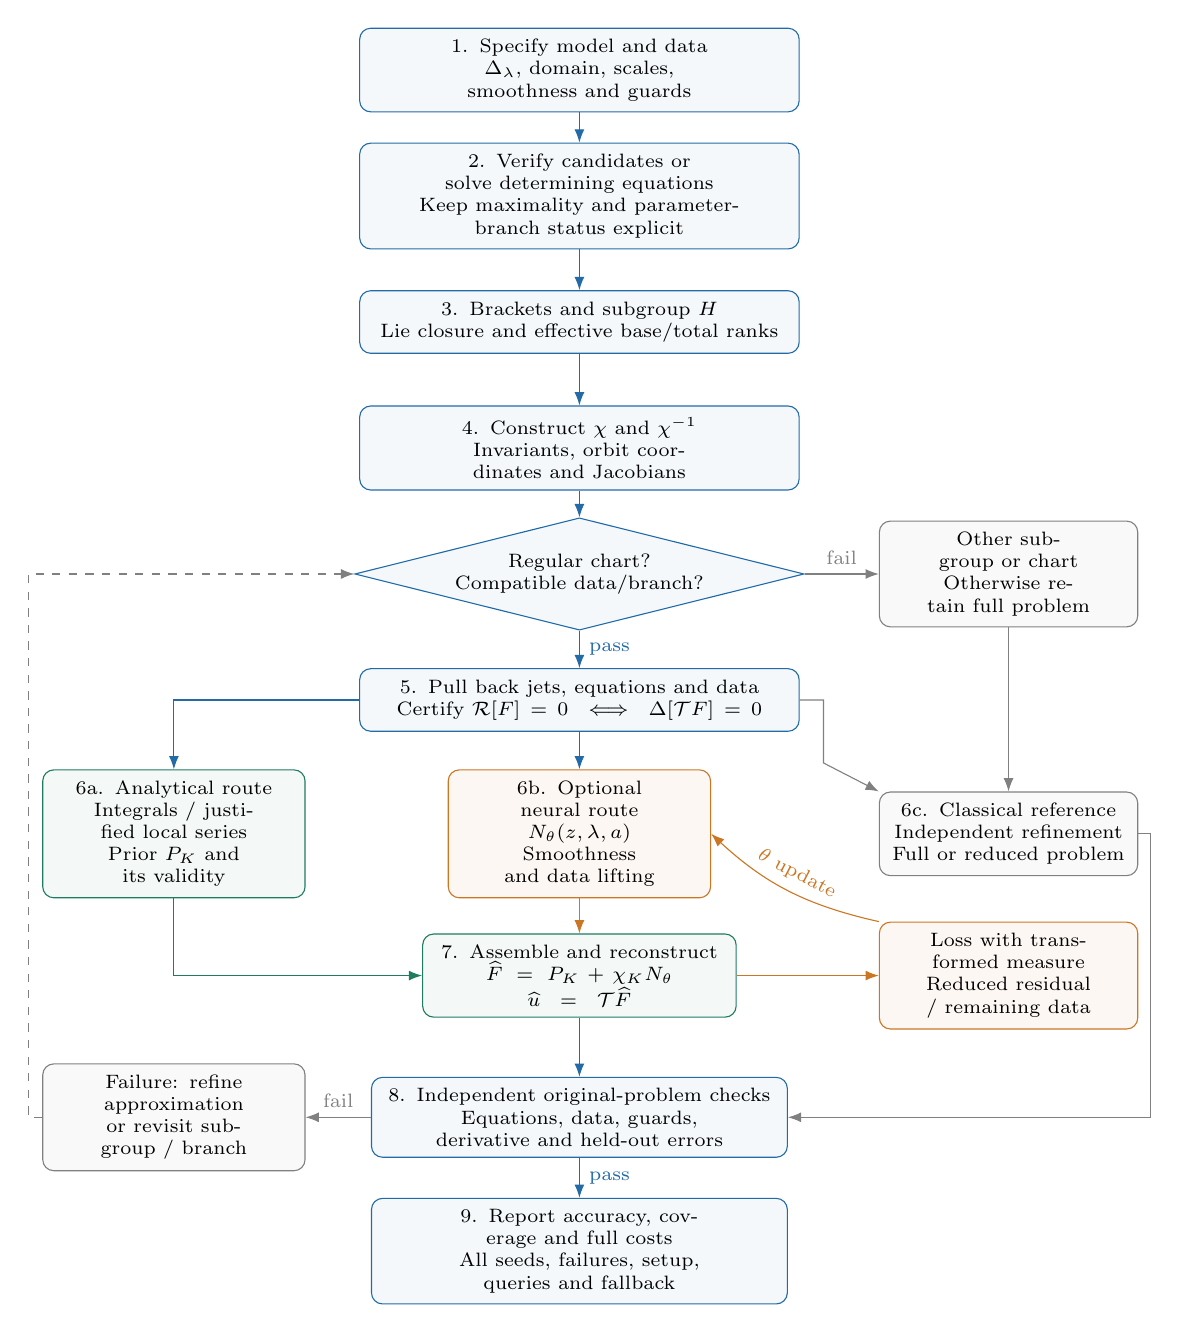
\begin{tikzpicture}[>=Latex,every node/.style={font=\scriptsize},
 box/.style={draw,rounded corners,align=center,inner sep=4pt,
             minimum height=.72cm},
 geom/.style={box,draw=fundgeometry,fill=fundgeometry!5},
 ana/.style={box,draw=fundanalysis,fill=fundanalysis!5},
 learn/.style={box,draw=fundlearning,fill=fundlearning!6},
 ref/.style={box,draw=gray,fill=gray!5}]
 \node[geom,text width=5.3cm] (model) at (5,0)
  {1. Specify model and data\\$\Delta_\lambda$, domain, scales, smoothness and guards};
 \node[geom,text width=5.3cm] (verify) at (5,-1.6)
  {2. Verify candidates or solve determining equations\\Keep maximality and parameter-branch status explicit};
 \node[geom,text width=5.3cm] (select) at (5,-3.2)
  {3. Brackets and subgroup $H$\\Lie closure and effective base/total ranks};
 \node[geom,text width=5.3cm] (chart) at (5,-4.8)
  {4. Construct $\chi$ and $\chi^{-1}$\\Invariants, orbit coordinates and Jacobians};
 \node[diamond,aspect=4,draw=fundgeometry,fill=fundgeometry!5,
       align=center,text width=3.3cm,inner sep=1pt] (guard) at (5,-6.4)
  {Regular chart?\\Compatible data/branch?};
 \node[ref,text width=3cm] (fallback) at (10.45,-6.4)
  {Other subgroup or chart\\Otherwise retain full problem};
 \node[geom,text width=5.3cm] (reduced) at (5,-8.0)
  {5. Pull back jets, equations and data\\Certify $\mathcal R[F]=0\iff\Delta[\mathcal TF]=0$};
 \node[ana,text width=3.05cm] (analytical) at (-.15,-9.7)
  {6a. Analytical route\\Integrals / justified local series\\Prior $P_K$ and its validity};
 \node[learn,text width=3.05cm] (neural) at (5,-9.7)
  {6b. Optional neural route\\$N_\theta(z,\lambda,a)$\\Smoothness and data lifting};
 \node[ref,text width=3cm] (reference) at (10.45,-9.7)
  {6c. Classical reference\\Independent refinement\\Full or reduced problem};
 \node[ana,text width=3.7cm] (assembly) at (5,-11.5)
  {7. Assemble and reconstruct\\$\widehat F=P_K+\chi_KN_\theta$\\$\widehat u=\mathcal T\widehat F$};
 \node[learn,text width=3cm] (loss) at (10.45,-11.5)
  {Loss with transformed measure\\Reduced residual / remaining data};
 \node[geom,text width=5cm] (check) at (5,-13.3)
  {8. Independent original-problem checks\\Equations, data, guards, derivative and held-out errors};
 \node[ref,text width=3.05cm] (refine) at (-.15,-13.3)
  {Failure: refine approximation\\or revisit subgroup / branch};
 \node[geom,text width=5cm] (report) at (5,-15.0)
  {9. Report accuracy, coverage and full costs\\All seeds, failures, setup, queries and fallback};
 \draw[->,fundgeometry] (model)--(verify);
 \draw[->,fundgeometry] (verify)--(select);
 \draw[->,fundgeometry] (select)--(chart);
 \draw[->,fundgeometry] (chart)--(guard);
 \draw[->,fundgeometry] (guard)--(reduced) node[midway,right] {pass};
 \draw[->,gray] (guard)--(fallback) node[midway,above] {fail};
 \draw[->,gray] (fallback)--(reference);
 \draw[->,fundgeometry] (reduced.west)-|(analytical.north);
 \draw[->,fundgeometry] (reduced)--(neural);
 \draw[->,gray] (reduced.east)--(8.1,-8.0)--(8.1,-8.8)--(reference.north west);
 \draw[->,fundanalysis] (analytical.south)|-(assembly.west);
 \draw[->,fundlearning] (neural)--(assembly);
 \draw[->,fundlearning] (assembly)--(loss);
 \draw[->,fundlearning] (loss.north west) to[bend left=15]
   node[midway,above,sloped] {$\theta$ update} (neural.east);
 \draw[->,fundgeometry] (assembly)--(check);
 \draw[->,gray] (reference.east)--(12.25,-9.7)--(12.25,-13.3)--(check.east);
 \draw[->,gray] (check)--(refine) node[midway,above] {fail};
 \draw[->,gray,dashed] (refine.west)--(-2,-13.3)--(-2,-6.4)--(guard.west);
 \draw[->,fundgeometry] (check)--(report) node[midway,right] {pass};
\end{tikzpicture}
\caption{Complete local reduction and approximation workflow. Blue denotes
exact geometry, green analysis, orange trainable approximation, and gray
independent references and failure routes. Parameter changes return to the
symmetry/chart checks; they do not merely become new network inputs.}
\label{fig:complete-workflow}
\end{figure}

\subsection{Where the neural optimization acts}
\label{sec:optimization-core}
For a verified reconstruction, the trainable variables are the profile
remainder coefficients $\theta$, unless a separate generator-learning
problem has been specified and certified. For fixed $\lambda,a$, use
\begin{equation}
 \widehat F_\theta=P_K+\chi_KN_\theta(z,\lambda,a),\qquad
 \widehat u_\theta=\mathcal T\widehat F_\theta,\qquad
 \mathcal L=\int\mathcal R[\widehat F_\theta]^T
                    W_H\mathcal R[\widehat F_\theta]\,dz
             +w_B\|\bar{\mathcal B}[\widehat F_\theta]\|^2.
 \label{eq:neural}
\end{equation}
Average over the declared parameter/data distribution when learning a
family. Add an observation term only when measurements are supplied.
If only zero-set equivalence is available, evaluate the original residual
pullback with its changed domain measure directly; do not assume a
factorization matrix or $W_H$ without verification.
If $W_H$ is fixed, the residual contribution to a directional gradient is
\begin{equation}
 D_\theta\mathcal L[\dot\theta]
  =2\int (D_F\mathcal R[\widehat F_\theta]
                    (\chi_KD_\theta N_\theta[\dot\theta]))^T
                      W_H\mathcal R[\widehat F_\theta]\,dz,
 \label{eq:optimization-gradient-core}
\end{equation}
plus remaining-data terms. Profile-dependent $W_H$ contributes its own
derivative. $D_F\mathcal R$ is a differential linearization, so the network
must supply the required field derivatives; reducing input dimension does
not remove the derivative budget or ensure good conditioning.

\begin{figure}[htbp]
\centering
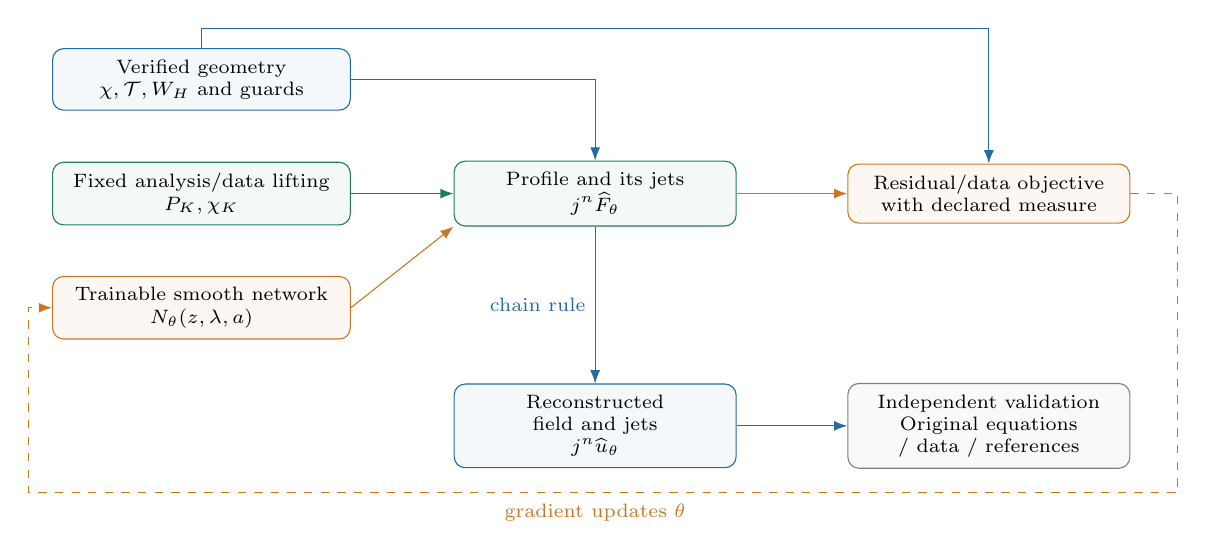
\begin{tikzpicture}[>=Latex,every node/.style={font=\scriptsize},
 box/.style={draw,rounded corners,align=center,inner sep=4pt,
             minimum height=.75cm}]
 \node[box,draw=fundgeometry,fill=fundgeometry!5,text width=3.5cm] (chart) at (0,0)
  {Verified geometry\\$\chi,\mathcal T,W_H$ and guards};
 \node[box,draw=fundanalysis,fill=fundanalysis!5,text width=3.5cm] (prior) at (0,-1.45)
  {Fixed analysis/data lifting\\$P_K,\chi_K$};
 \node[box,draw=fundlearning,fill=fundlearning!6,text width=3.5cm] (net) at (0,-2.9)
  {Trainable smooth network\\$N_\theta(z,\lambda,a)$};
 \node[box,draw=fundanalysis,fill=fundanalysis!5,text width=3.3cm] (profile) at (5,-1.45)
  {Profile and its jets\\$j^n\widehat F_\theta$};
 \node[box,draw=fundlearning,fill=fundlearning!6,text width=3.3cm] (loss) at (10,-1.45)
  {Residual/data objective\\with declared measure};
 \node[box,draw=fundgeometry,fill=fundgeometry!5,text width=3.3cm] (physical) at (5,-4.4)
  {Reconstructed field and jets\\$j^n\widehat u_\theta$};
 \node[box,draw=gray,fill=gray!5,text width=3.3cm] (checks) at (10,-4.4)
  {Independent validation\\Original equations / data / references};
 \draw[->,fundanalysis] (prior)--(profile);
 \draw[->,fundlearning] (net.east)--(profile.south west);
 \draw[->,fundgeometry] (chart.east)--(5,0)--(profile.north);
 \draw[->,fundgeometry] (chart.north)--(0,.65)--(10,.65)--(loss.north);
 \draw[->,fundlearning] (profile)--(loss);
 \draw[->,fundlearning,dashed] (loss.east)--(12.4,-1.45)--(12.4,-5.25)
   --(-2.2,-5.25)--(-2.2,-2.9)--(net.west);
 \node[fundlearning] at (5,-5.5) {gradient updates $\theta$};
 \draw[->,fundgeometry] (profile)--(physical) node[midway,left] {chain rule};
 \draw[->,fundgeometry] (physical)--(checks);
\end{tikzpicture}
\caption{Parallel inputs to a constrained profile and its optimization.
The fixed geometric maps and analytical prior enter the forward calculation;
the gradient loop updates the neural remainder. Independent original-field
checks do not replace the training loss or the required stability analysis.}
\label{fig:network-parallel}
\end{figure}

\clearpage
\section{Examples: interpretation, verification and the SVE benchmark}
\label{sec:examples}
The examples illustrate the preceding contract; none is a hypothesis of the
general theorems. A verified reduction describes a selected invariant family,
and every chart and data restriction is retained.

\begin{example}[A nonlinear PDE can reduce to either a PDE or an ODE]
For viscous Burgers, $u_t+uu_x=\nu u_{xx}$, $\nu>0$, select
$X=\partial_t+c\partial_x$. The complete adapted chart is
$y=t$, $z=x-ct$, $v=u$, with inverse $t=y$, $x=z+cy$, $u=v$.
Its base Jacobian is one, $Xy=1$, $Xz=Xv=0$, and graph invariance is
$u_t+cu_x=0$. Thus $u=F(z)$ and direct substitution gives
\[
 \nu F''+(c-F)F'=0.
\]
Here $p=2$, $\ell=1$, $d=1$, and the second differential order is retained.
In contrast, for $u_t=\nu(u_{xx}+u_{ww})+u(1-u)$, invariance under
$\partial_w$ gives $u=V(t,x)$ and a nonlinear PDE in two variables.
Adding the commuting generator $\partial_t+c\partial_x$ gives
\[
 \nu F''+cF'+F(1-F)=0.
\]
The successive quotient dimensions are two and one. Effective orbit rank
decides the number of profile arguments in these nonlinear examples.
\end{example}

\begin{example}[Infinite point algebras, including a nonlinear example]
For $u_t=u_{xx}$, every solution $f_t=f_{xx}$ gives a point generator
$f(t,x)\partial_u$ through linear superposition. This is an
infinite-dimensional abelian ideal in the point algebra, distinct from its
finite-dimensional essential quotient \cite{koval2023}.
For the nonlinear Liouville equation $w_{xy}=e^w$, arbitrary smooth
functions $A(x)$ and $B(y)$ generate
\[
 X=A(x)\partial_x+B(y)\partial_y
                  -(A'(x)+B'(y))\partial_w.
\]
Indeed, for $\Delta=w_{xy}-e^w$,
$\pr^{(2)}X\Delta=-(A'+B')\Delta$. The finite local action can be written
$\bar x=f(x)$, $\bar y=h(y)$,
$\bar w=w-\log(f'h')$ on a branch $f'h'>0$. This verifies arbitrary-function
point symmetry directly; nonlinear PDEs need not have finite point algebras
\cite{levi2015}. Selecting a finite-dimensional regular subgroup remains
possible in either example.
\end{example}

\begin{example}[A parameter stratum can change symmetry dimension]
For $u_t-u_{xx}-\mu u^2=0$, a vertical shift candidate
$f(t,x)\partial_u$ has infinitesimal residual
$f_t-f_{xx}-2\mu uf$. At $\mu=0$, every heat solution supplies a symmetry.
At $\mu\ne0$, the freedom in $u$ forces $f=0$ in this particular vertical
shift class. This verifies loss of that ideal; it does not by itself classify
the remaining algebra. Exceptional parameter strata and the declared
symmetry class must both accompany a symmetry count.
\end{example}

\begin{example}[The published scalar Lagrangian benchmark]
\label{ex:sve}
Paliathanasis, Leon and Leach \cite{ap} report the scalar equation
\begin{equation}
 \E_m[\phi]=D_t\!\left(\phi_s\phi_{tt}
                       -g\frac{\phi_{ss}}{\phi_s^2}\right)
 -g\beta_{\rm tr}D_s\!\left(\phi_t^{m-1}
                                 \frac{\phi_{ts}}{\phi_s}\right)=0,
 \qquad \beta_{\rm tr}=m\kappa,\quad \kappa=A_g\xi_{\rm por}.
 \label{eq:sve}
\end{equation}
Here $(t,s)$ are time and material-label coordinates and $\phi$ is particle
position. The porosity factor $\xi_{\rm por}$ is not a generator coefficient
$\xi^i$; the porosity itself is also distinct from the group parameter
$\varepsilon$. We audit the printed scalar equation as a mathematical
benchmark. Its equivalence to the full physical bed-transport system is a
separate question addressed below. The positive branch $\phi_s>0$ permits
$h=1/\phi_s$; noninteger powers additionally require a stated real branch
for $\phi_t$.
\end{example}

\subsection{What the reference includes, and what must be made explicit here}
The reference is a model-specific Lie calculation, not a general reduction
theorem. Its equations (9)--(12) give the point action and generator,
(13)--(18) the infinitesimal test/prolongation and determining system,
(22)--(23) the invariant equations, and Table 3 the similarity variables.
Thus the coordinate transformation is present, mainly through invariants
and an ansatz. It does not write out all orbit coordinates, inverse maps,
Jacobians, data pullbacks or residual measures needed for a reusable solver.
Its citations provide the general background; our general results above
state their hypotheses and local scope explicitly and credit that background.

\begin{center}\small
\renewcommand{\arraystretch}{1.12}
\begin{tabularx}{\linewidth}{@{}p{3.6cm}p{3.8cm}X@{}}
\toprule
Reference object/location & Unified notation & Extra verification in this paper \\
\midrule
$(t,s,\phi)$; equation (7) & $(x,u)$; $\Delta=\E_m$ & Fixed parameters, denominator and real-power branches. \\
$X$; equations (9)--(12) & $X_b$, $Q_b$ & Equation symmetry versus invariant solution graph. \\
$X^{[n]}$; equations (13)--(18) & $\pr^{(n)}X$ & Explicit jet chain rule and multiplier/zero-set check. \\
$W^{[0]},W^{[1]}$; equations (22)--(23), Table 3 & $z,v$ & Complete $(y,z,v)$ chart, inverse and ranks. \\
Similarity ansatz/reduced equations & $u=\mathcal TF$, $\mathcal R[F]=0$ & Independent substitution, data and norm pullbacks. \\
Proposition 1, Tables 1--2 & $\mathfrak g_\lambda$, brackets, adjoint action & Attribution of classification; convention and consistency audit. \\
\bottomrule
\end{tabularx}
\end{center}

The printed source also needs careful reading. Under the bracket convention
$[X,Y]=XY-YX$, its Table 1 gives the same sign for both
$[X_1,X_5]$ and $[X_5,X_1]$, and similarly for the $X_2,X_5$ pair.
Direct computation instead gives
\[
 [\partial_t,X_5]=\partial_t,\quad [X_5,\partial_t]=-\partial_t,
 \qquad [\partial_s,X_5]=-2\partial_s,\quad
 [X_5,\partial_s]=2\partial_s.
\]
The text of its stationary subsections 3.1--3.2 interchanges the surviving
variables, although Table 3 gives them correctly: $X_1=\partial_t$ yields
$\phi=F(s)$, and $X_2=\partial_s$ yields $\phi=F(t)$.
A pure vertical translation $X_3=\partial_\phi$ has $Q=1$ and hence no
fixed scalar solution graph. These checks concern specific printed entries,
not a new maximal-classification proof. In particular, we verify our reduced
equation by substitution rather than importing equation (25) as an identity.

The displayed determining system on the reference's page 4 contains
$3\eta^1+\xi^2_{,s}+2\xi^1_{,t}=0$. Its reported scaling generator
$X_4$ has $\eta^1=1$, $\xi^1=t$, $\xi^2=s$, giving $6=0$ in that
printed condition. This identifies an internal inconsistency, potentially
typographical; it does not invalidate a generator independently verified
against the original scalar residual. The printed determining system must
be corrected and solved before it can support a maximality proof.

\subsection{The complete exceptional-branch coordinate transformation}
At $m=3$ the source reports the additional generator
$X_5=t\partial_t-2s\partial_s$. Its finite flow is
$(t,s,\phi)\mapsto(e^\varepsilon t,e^{-2\varepsilon}s,\phi)$.
On $t>0$, with a fixed reference time $t_*>0$, choose
\begin{equation}
 y=\log(t/t_*),\quad z=st^2,\quad v=\phi;
 \qquad t=t_*e^y,\quad s=z/t^2,\quad \phi=v.
 \label{eq:sve-chart}
\end{equation}
Then $X_5y=1$, $X_5z=X_5v=0$,
$\det D_{(t,s)}(y,z)=t\ne0$, and the fibre Jacobian is one.
With $v=F(z)$ the reconstruction is $\phi(t,s)=F(st^2)$, and
\begin{equation}
 \partial_t=\frac1t(\partial_y+2z\partial_z),\qquad
 \partial_s=t^2\partial_z,
 \qquad
 \phi_s=t^2F',\quad \phi_t=\frac{2zF'}t,
 \quad \phi_{tt}=\frac{2zF'+4z^2F''}{t^2}.
 \label{eq:sve-chain-rule}
\end{equation}
The prime denotes $d/dz$ throughout this example. Direct substitution gives
\begin{align}
 \E_3[F(st^2)]&=\frac1t\mathcal R_0[F],\qquad
 \mathcal R_0[F]=2z\mathcal A'[F]-g\beta_{\rm tr}\mathcal B'[F],\label{eq:reduction}\\
 \mathcal A[F]&=2z(F')^2+4z^2F'F''-g\frac{F''}{(F')^2},\qquad
 \mathcal B[F]=8z^2F'(F'+zF'').\nonumber
\end{align}
The off-shell multiplier $1/t$ is nonzero on this chart. The coefficient of
$F'''$ is
\begin{equation}
 c_{\rm lead}(z,F')=-\frac{2gz}{(F')^2}
                       +8(1-g\beta_{\rm tr})z^3F'.
 \label{eq:sve-leading}
\end{equation}
Use a third-order normal-form IVP only where $F'>0$ and
$c_{\rm lead}\ne0$. For $1-4g\beta_{\rm tr}>0$, the explicit branch
\begin{equation}
 F_0(z)=C+Kz^{1/3},\qquad K^3=\frac{27g}{1-4g\beta_{\rm tr}}
 \label{eq:sve-exact}
\end{equation}
solves the verified scalar equation on $z>0$ and supplies an exact check.
It is not an existence theorem for arbitrary physical initial/boundary data.

\begin{center}
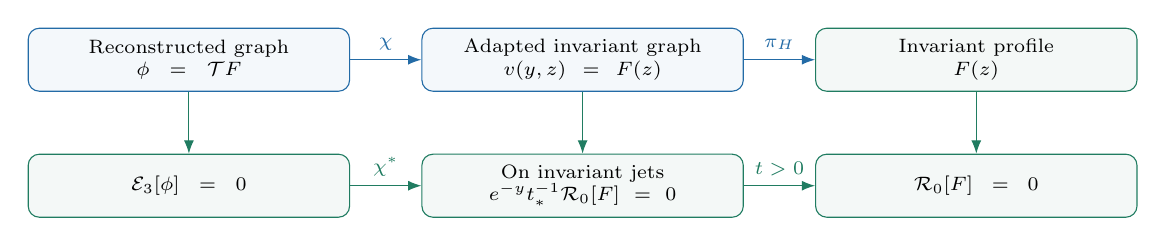
\begin{tikzpicture}[>=Latex,every node/.style={font=\scriptsize},
 box/.style={draw,rounded corners,align=center,text width=3.8cm,
              minimum height=.8cm,inner sep=4pt}]
 \node[box,draw=fundgeometry,fill=fundgeometry!5] (original) at (0,0)
  {Reconstructed graph\\$\phi=\mathcal TF$};
 \node[box,draw=fundgeometry,fill=fundgeometry!5] (adapted) at (5,0)
  {Adapted invariant graph\\$v(y,z)=F(z)$};
 \node[box,draw=fundanalysis,fill=fundanalysis!5] (profile) at (10,0)
  {Invariant profile\\$F(z)$};
 \node[box,draw=fundanalysis,fill=fundanalysis!5] (pde) at (0,-1.6)
  {$\E_3[\phi]=0$};
 \node[box,draw=fundanalysis,fill=fundanalysis!5] (factor) at (5,-1.6)
  {On invariant jets\\$e^{-y}t_*^{-1}\mathcal R_0[F]=0$};
 \node[box,draw=fundanalysis,fill=fundanalysis!5] (ode) at (10,-1.6)
  {$\mathcal R_0[F]=0$};
 \draw[->,fundgeometry] (original)--(adapted) node[midway,above] {$\chi$};
 \draw[->,fundgeometry] (adapted)--(profile) node[midway,above] {$\pi_H$};
 \draw[->,fundanalysis] (pde)--(factor) node[midway,above] {$\chi^*$};
 \draw[->,fundanalysis] (factor)--(ode) node[midway,above] {$t>0$};
 \draw[->,fundanalysis] (original)--(pde);
 \draw[->,fundanalysis] (adapted)--(factor);
 \draw[->,fundanalysis] (profile)--(ode);
\end{tikzpicture}
\end{center}

For the chart domain $1\le t\le2$, $1\le z\le1.5$, take $t_*=1$.
The inverse base Jacobian is $1/t=e^{-y}$ and the residual multiplier is
$e^{-y}$. Thus the unnormalized original squared-residual integral equals
\[
 \int_{\Omega}|\E_3[\mathcal TF]|^2\,dt\,ds
   =\frac7{24}\int_1^{1.5}|\mathcal R_0[F](z)|^2\,dz.
\]
Normalized averages require their own domain-volume factors. This example
shows why the quotient loss measure must be declared rather than inferred
from the invariant coordinate alone.

\subsection{Physical-model audit before any full-SVE interpretation}
Let $B(t,x)$ be Eulerian bed elevation and $b(t,s)=B(t,\phi(t,s))$ its
material pullback. Suppose the Eulerian transport equation is
$B_t+\beta_{\rm tr}u^{m-1}u_x=0$, with $u(t,\phi)=\phi_t$.
The chain rule gives
\begin{equation}
 b_t=B_t+\phi_tB_x,\qquad b_s=\phi_sB_x,
 \qquad
 b_t-\frac{\phi_t}{\phi_s}b_s
       +\beta_{\rm tr}\phi_t^{m-1}\frac{\phi_{ts}}{\phi_s}=0.
 \label{eq:physical-bed-audit}
\end{equation}
The source's printed equation (6) lacks this advective bed term when its bed
variable is interpreted as the Eulerian pullback. A different variable or
closure would have to be defined to justify its omission. Consequently the
scalar benchmark, its reported symmetry classification, and a physically
equivalent full SVE reduction cannot be treated as interchangeable. Resolve
this derivation with the authors/source model before making the latter claim;
changing the model also requires a new symmetry and data calculation.
Smooth classical reductions here do not establish shock solutions or weak
Rankine--Hugoniot balances.

There is also an integration issue even for the source's printed model.
Set $A=\phi_s\phi_{tt}-g\phi_{ss}/\phi_s^2$ and
$C=\phi_t^{m-1}\phi_{ts}/\phi_s$. Its equations (5)--(6) require
$b_s=-A/g$ and $b_t=-\beta_{\rm tr}C$. Thus the one-form
\[
 \omega=-\beta_{\rm tr}C\,dt-\frac{A}{g}\,ds
\]
is closed precisely when $\mathcal E_m[\phi]=0$. On a sufficiently small
simply connected regular domain, the Poincare lemma reconstructs $b$ up to
an additive constant. On a multiply connected domain, vanishing periods
are additionally necessary. Prescribed bed data must agree with this
primitive. This recovers only the printed two-equation model; it does not
repair the missing advective term in the physical pullback. A scalar PDE
certificate and a physical full-system certificate are therefore distinct.

\subsection{Persistence and the limitations of a near-cubic ansatz}
For the printed scalar equation, weighted prolongation gives the off-shell
identity
\begin{equation}
 \pr^{(3)}X_5\E_m+\E_m
  =(m-3)g\beta_{\rm tr}D_s\!\left(
        \phi_t^{m-1}\frac{\phi_{ts}}{\phi_s}\right).
 \label{eq:sve-defect}
\end{equation}
It verifies $X_5$ at $m=3$ and exhibits its generic defect away from that
stratum. For a regular branch at $m=4$ the right-hand side is generically
nonzero on shell. Failure of a guessed multiplier alone would not prove
this; the explicit on-shell defect does. Persistence of a \emph{deformed}
generator remains a separate determining-system question.
Use equation~\eqref{eq:first-order-core} before extending this chart to
$m=3+\delta$. In a nondimensional model, vary $m$ at fixed nondimensional
$\kappa$ and retain $\beta_{\rm tr}=m\kappa$. A logarithmic expansion uses a
positive dimensionless velocity $\phi_t/U_*$; a logarithm of a dimensional
velocity does not define a constitutive perturbation.
If no continued symmetry is verified, an unrestricted field correction
satisfies a linearized PDE of the form
\[
 D_\phi\E_0[\mathcal TF]\psi+\E_1[\mathcal TF]=0.
\]
Writing $\psi=F_1(st^2)$ without checking closure would impose an unsupported
reduction. A prescribed time-dependent transport coefficient, or physical
time-dependent data, each requires its own model/symmetry/data audit.
The next ML experiment below therefore varies a data parameter at fixed
$m=3$, while near-cubic continuation remains mathematical work.


\clearpage
\section{Related work and research position}
Symmetry-informed neural solution methods already exist. Akhound-Sadegh
et al.\ \cite{sympinn} penalize infinitesimal changes of the PDE residual;
this does not require every predicted solution to satisfy $Q=0$.
Jiao and Xiong \cite{jiao} exploit symmetry conditions for fundamental
solutions of linear PDEs. Kavousanakis et al.\ \cite{flow} learn time-varying
moving or rescaled coordinates and profiles through a PINN coupled to
index-2 differential-algebraic constraints; their examples include nonlinear
wave and spreading equations. LieSolver builds PDE solutions from known
symmetry transformations and fits initial/boundary data, but its reported
scope is linear homogeneous PDEs \cite{liesolver}. Lie point symmetry data
augmentation (LPSDA) transforms known solution data to improve the sample
complexity of neural PDE solvers \cite{lpsda}; it is not an exact quotient or
a symmetry-discovery certificate. Generalized-symmetry loss augmentation has
also been proposed for physics-informed neural operators when ordinary point
symmetries provide little training signal \cite{genliepino}. Thus combining Lie
information and neural PDE solvers is not a novelty claim. A one-dimensional SVE Lie analysis
also predates this study, and the selected Lagrangian source already reports
its symmetry algebra and similarity reductions \cite{sveold,ap}; discovery of
SVE symmetries or of $X_5$ is not claimed. The proposed contribution is
independent verification, persistence or obstruction under parameter
perturbation, and a parameter-conditioned neural correction to a reduced
analytical profile. Otto et al.'s 2025 review unifies symmetry enforcement,
discovery, and promotion through Lie-derivative constraints; LieLAC uses
infinitesimal generators to canonicalize inputs for pre-trained models,
including neural PDE solvers \cite{otto,lieLAC}. These offer useful ML
interfaces, while the direct low-cost path here is exact symmetry reduction
before training. A 2025 master's thesis provides a recent worked account of
determining equations, gas-dynamic PDE systems, and symmetry-compatible
initial-boundary data \cite{beligiannis}. Tarayrah, Pitzel and Cheviakov
compare BGI and FS approximate symmetries for nonlinear PDEs, prove relations
only under stated hypotheses, exhibit classification differences, and separate
symmetry classification from approximate-solution and wave-breaking accuracy
\cite{tarayrah2023}. Their results rule out a single undifferentiated label
``approximate symmetry found.'' The 2024 algorithmic study of approximate
symmetry algebras instead defines an approximate algebra through an exact
algebra of a nearby equation; it highlights involutive completion and warns
that numerical rank/SVD results can depend on base point and tolerance
\cite{approxalg}. An SDE preprint cited in the supplied draft learns generators while enforcing
Lie-bracket closure; this is adjacent evidence for learning algebra structure,
not a PDE classification result \cite{liestonet}. Effectiveness remains an
experimental question.

The supplied sources sharpen the scope of the classification claim. Liu and
Lou's 2024 review treats classical point reduction, conditional and CK-direct
methods, finite transformation groups, nonlocal methods, and supersymmetry as
distinct constructions; these should not be merged into one ``complete Lie
algebra'' \cite{liulou}. The supplied 2017 MSc dissertation works through
classical point reductions and nonclassical symmetries for drift-diffusion,
biased-diffusion, and KiSS population PDEs \cite{mathebula}. Hijazi's 2013 PhD
thesis compares classical, nonclassical, and potential-symmetry workflows on
coupled systems, including Burgers-type models, and discusses special cases
and time-dependent coefficients \cite{hijazi}. These are useful procedural
examples, but neither thesis is evidence for a new SVE result or a 2024--2026
ML method. For the low-cost study, complete the classical local
point-algebra calculation if maximality is claimed; pursue conditional, potential/nonlocal, or other
symmetry notions only as separately named extensions motivated by the target
model and available conservation laws.

\clearpage
\section{Publication review: claims, missing proofs and evidence gates}
\label{sec:publication-review}
The standard local reduction theorems above make the mathematical argument
auditable; they do not constitute the paper's research novelty. Publication
needs one explicit new result with a comparison and evidence appropriate to
that claim. The present paper is theorem-first: its primary target is an
unrestricted regular continuation or certified first obstruction for the
exceptional near-cubic point-symmetry generator. The existing diagonal-scaling
P0 certificate is evidence in a restricted class, not that theorem. A reusable
exact/BGI/FS/nearby-equation benchmark is supporting infrastructure, and
real-world shallow-water demonstrations are validation or follow-on studies.
The present manuscript remains a research draft with verified local identities,
historical numerical reports, and a proposed next experiment. Proofreading
alone cannot convert these into a completed research result.

\begin{center}\small
\renewcommand{\arraystretch}{1.14}
\begin{tabularx}{\linewidth}{@{}p{3.1cm}XX@{}}
\toprule
Issue & Required formal action & Claim allowed after the action \\
\midrule
Contribution and attribution & Prove unrestricted regular parameter continuation through a declared order or certify the first obstruction order. Credit existing SVE classification and symmetry-informed neural PDE work. & A specific new continuation/obstruction proposition; not discovery of $X_5$, not a conclusion extrapolated from the scaling ansatz, and not universal Lie--ML novelty. \\
Model interpretation & Resolve equation~\eqref{eq:physical-bed-audit}; define units, bed variable, closure and parameter convention. & Physical SVE interpretation only for the derived model. Until then, the printed scalar benchmark. \\
Reduction proof & Retain inverse/Jacobian checks, branch guards, equation equivalence, pulled-back data and reconstruction. Cover or list every excluded stratum. & Local invariant solutions on the stated branch; not all solutions or a global classification. \\
Classifications and tables & Distinguish source classification, finite-ansatz verification and maximality. Recompute brackets with a declared convention. & Precisely stated algebra coverage and subgroup selection. \\
Existence, error and stability & Prove normal-form IVP conditions; add uniform stability and residual/quadrature bounds for any error-certificate claim. & Numerical accuracy without a certificate, or a conditional theorem with all its hypotheses. \\
Numerical evidence & Recover matching code, configurations, raw histories, seeds, references and machine information. Separate new runs from historical tables. & Reproducible measured performance within the declared experiment. \\
Scope and presentation & Keep general theory before Examples, isolate speculative scale bridges, use consistent symbols and a self-contained bibliography. & A readable paper with a bounded mathematical and experimental scope. \\
\bottomrule
\end{tabularx}
\end{center}

The newly adopted contract is theorem-first: establish unrestricted regular
persistence through a declared order or certify the first obstruction on a
stated parameter branch, then derive any admissible reduced problem and its
local analytical expansion. The verified fixed branch may still support a
secondary controlled test of whether an equation-derived prior improves error
versus time, but that protocol is not the paper's primary claim. It still needs
the reduction/data proofs and must not present a numerical comparison as a
general sample-complexity theorem. If maximal symmetry classification is a
claimed contribution, the full determining system and its parameter/singular
branches must be completed; a useful supplied subgroup does not require that
stronger claim.

The attached reference's compact presentation explains why several general
theorems are implicit there. For this paper's reusable method, the missing
links are exactly the explicit hypotheses and maps in
Section~\ref{sec:general-core}, rather than additional unrelated examples.
An interval-wide analytical conclusion needs uniform bounds, not merely
regularity sampled on a mesh. Fractional/nonlocal operators and weak/shock
solutions are extensions with separate analytical contracts.

\section{Next ML experiment: a controlled test on a verified data family}
\label{sec:next-experiment}
This section preserves a secondary prospective protocol, not a report of new
training runs and not the theorem-first paper's primary experiment. Its local
question is whether a fourth-order equation-derived prior improves the learned
family beyond the quadratic polynomial already needed to impose a third-order
IVP's data. A separate comparison tests the benefit of restricting the field
to the verified invariant coordinates. These runs remain gated until the
unrestricted continuation/obstruction analysis is reported or explicitly
separated as fixed-branch supporting evidence.

\subsection{Mathematical and reference-solution prerequisites}
Use the nondimensional printed scalar benchmark at
$m=3$, $g=1$, $\beta_{\rm tr}=0.1$, $\kappa=0.1/3$.
Keep $\delta=m-3=0$. On $z\in[1,1.5]$ and $t\in[1,2]$, let
$K=\sqrt[3]{45}$ and vary only the data parameter $a\in[-0.02,0.02]$:
\begin{equation}
 F(1;a)=K,\qquad F'(1;a)=K/3,\qquad
 F''(1;a)=-2K(1+a)/9.
 \label{eq:experiment-ivp}
\end{equation}
The corresponding original data on $\Gamma_0=\{st^2=1\}$ are
\begin{equation}
 \phi=K,\qquad t^{-2}\phi_s=K/3,\qquad
 t^{-4}\phi_{ss}=-2K(1+a)/9.
 \label{eq:experiment-original-data}
\end{equation}
Their prolonged $X_5$ action vanishes, and their pullbacks give
equation~\eqref{eq:experiment-ivp}. This is a constructed compatible data
family, not a physically sourced canal boundary problem. At $a=0$ the exact
profile~\eqref{eq:sve-exact} supplies a check. Normal-form existence and
continuous parameter dependence give a neighborhood of a regular solution;
the entire proposed interval/domain still needs verified guard bounds or a
clearly labeled numerical regularity check.

Before training, regenerate the exact chart, pullback and data certificates
from available source. Recover the newer generic backend only if its
capabilities are claimed. For every reference profile record
$\min F'$, $\min|c_{\rm lead}|$, chart/domain exits and independent solver
agreement. Solve all 17 distinct parameter cases below with DOP853 at
$(\mathrm{rtol},\mathrm{atol})=(10^{-9},10^{-12})$,
$(10^{-11},10^{-14})$, and $(10^{-13},10^{-15})$, and cross-check with Radau.
For the proposed $10^{-5}$ profile-error target, require at most $10^{-8}$
reference discrepancy on the evaluation grid. If guards fail, split or
shrink the family before training and disclose the change. Finite mesh
checks are not a uniform interval certificate.

For an analytical certificate on this reduced IVP, use
Proposition~\ref{prop:ode-error-core} with a verified regular tube,
a bound on $D_YG$, the leading-factor margin and a continuous residual
bound. These are additional deliverables beyond solver agreement.

Write the regular ODE as $F'''=G(z,F,F',F'')$. With $h=z-1$, define
\begin{align}
 P_2(z,a)&=K+(K/3)h-K(1+a)h^2/9,\\
 P_4(z,a)&=P_2+c_3(a)h^3+c_4(a)h^4,\label{eq:experiment-priors}\\
 c_3&=G(1,Y_0)/6,\qquad
 c_4=\bigl(G_z+F'G_F+F''G_{F'}+G\,G_{F''}\bigr)(1,Y_0)/24,\nonumber
\end{align}
where $Y_0=(F(1),F'(1),F''(1))$. Verify this recurrence symbolically and
against the exact $a=0$ series. Choosing $P_4$ does not prove that its
truncation is accurate over the whole training interval.

\subsection{Ablations that actually isolate the analytical prior}
\begin{center}\small
\renewcommand{\arraystretch}{1.16}
\begin{tabularx}{\linewidth}{@{}p{3cm}p{5.1cm}X@{}}
\toprule
Arm & Trial function & Question isolated \\
\midrule
B: reduced hard-IVP PINN & $\widehat F=P_2+h^3N_\theta(z,a)$ & Baseline with exactly the same three initial data. \\
H: added analytical prior & $\widehat F=P_4+h^3N_\theta(z,a)$ & Extra equation-derived coefficients with the same remainder factor and neural architecture. \\
H5: extra hard series jets & $\widehat F=P_4+h^5N_\theta(z,a)$ & Additional exact Taylor constraints and different conditioning; a separate ablation. \\
D: direct PDE PINN & $\widehat\phi=P_2(st^2,a)+(st^2-1)^3N_\theta(t,s,a)$ & Same supplied data, without imposing $Q_5=0$ on the trainable field. \\
Controls & $P_2$, $P_4$, exact $a=0$ profile; converged classical solver & Accuracy and total cost without neural training. \\
\bottomrule
\end{tabularx}
\end{center}

A ``hard-IVP PINN without an analytical part'' is misleading here: imposing
three data jets already builds $P_2$ into the trial function. Moreover B and H
have the same unconstrained smooth profile class up to a shift of the neural
remainder by $c_3+c_4h$; any observed advantage concerns the chosen finite
network, initialization and optimization, not elimination of unknown
degrees of freedom by $P_4$. H5 adds stronger exact local information and
must not be used alone to attribute an improvement to the prior.
The direct arm knows the supplied surface $st^2=1$ through its data lifting;
it is not a baseline with no information about the data geometry.

For the fixed cubic benchmark, equation~\eqref{eq:sve-defect} implies
$\pr^{(3)}X_5\E_3=-\E_3$. Squaring that Lie derivative of the residual
merely reweights the original squared-residual loss. It provides no
independent symmetry information in this case. A graph penalty
$\|Q_5[\widehat\phi]\|^2$, or a genuinely different symmetry-informed
baseline, must be named separately from the residual-Lie-derivative
construction of \citet{sympinn}. Exact reduction imposes $Q_5=0$ by
construction, but restricts the solution family.

In the full adapted PDE, the coefficient of the highest normal derivative
$v_{zzz}$ on the initial surface is $c_{\rm lead}/t=2K/t\ne0$ for these
data. The equation is analytic on the regular branch. The
Cauchy--Kowalevski theorem therefore supplies local existence and uniqueness
for the analytic data, consistently with the reconstructed analytic ODE
solution. This is a local analytic statement. A common domain reaching
$z=1.5$, smooth-problem stability and an error bound for approximate fields
still need their own analysis. Limit the numerical comparison to the stated
regular reference branch until those stronger claims are justified.

\paragraph{Classical approximation and launch criteria.}
Alongside the classical IVP solver, include a tensor-product Chebyshev
approximation or spline interpolant in $(z,a)$, built from declared
reference data. Report its label-generation cost separately from the
label-free residual training of B/H. This comparator tests whether a neural
family surrogate is useful beyond ordinary smooth interpolation; it is
not a matched zero-label baseline. Also retain an adaptive Taylor or
polynomial approximation of each profile to separate neural benefit from
the benefit of the analytical expansion itself.

Training starts only after (i) the exact scalar model and branch are frozen,
(ii) symbolic reconstruction and data checks are reproducible,
(iii) the reference family passes the declared convergence and guard tests,
and (iv) the loss measure, validation split, primary metric and cost
accounting are fixed. These gates authorize an empirical scalar-benchmark
experiment. A certified experiment additionally requires interval-wide
solution-tube and continuous-residual bounds; a physical SVE experiment
additionally requires resolving the bed-transport derivation. Neither
requirement is supplied by a small sampled training loss.

\subsection{Splits, optimization budget and smoothness}
Use disjoint data-parameter sets, with the final test set reserved before
hyperparameter selection:
\begin{align*}
 \mathcal T_a&=\{-0.02,-0.015,-0.01,0,0.01,0.015,0.02\},\\
 \mathcal V_a&=\{-0.0125,-0.005,0.005,0.0125\},\\
 \mathcal S_a&=\{-0.018,-0.008,-0.002,0.002,0.008,0.018\}.
\end{align*}
The older draft used $\mathcal V_a$ as held-out cases; they therefore cannot
serve as a newly untouched final test. Symmetry-generated orbit copies stay
in the same split. Training uses no interior reference-solution labels;
validation and test references still count toward setup cost.

Use float64 and smooth $\tanh$ networks so the third-order original residual
and optimization derivatives exist. A pilot architecture with two hidden
layers of width 24 has 697 parameters for input $(z,a)$ and 721 for
$(t,s,a)$; report these counts rather than claiming identical budgets.
Use fixed affine input scaling from the declared domains, including
$\widetilde z=4z-5$ and $\widetilde a=a/0.02$; compute physical residual
derivatives with all inverse scaling factors. Pair B/H initializations and
collocation seeds so their primary difference is the analytical prior.
Start with B, H and D, seeds 0 and 1, 128 residual points per training
parameter and 1000 Adam updates at learning rate $10^{-3}$. Sample the
direct arm in $(t,z)$ and transform to $(t,s)$ with the correct quadrature
weight. Draw independent collocation coordinates using the same declared
sampler. If the pilot passes the mathematical/reference and numerical
finiteness gates, confirm with seeds 0--4 at 64, 128 and 256 points per
parameter. Test H5 only as the separately declared ablation. Run sequentially
within the available CPU or 6 GB GPU budget and record the actual hardware.

This pilot budget is a starting protocol, not an assertion of adequate
capacity or convergence. Use $\mathcal V_a$ for any documented budget or
conditioning adjustment, freeze the final configurations before opening
$\mathcal S_a$, and retain all seeds and failures. Report both matched-step
comparisons and error versus measured time. The original-volume objective
for B/H can be evaluated using the factor $7/24$ above; normalized objectives
use the corresponding volume. Use the same fixed nondimensional residual
scales across arms, not method-dependent denominators chosen after training.
Distinct quotient states, original-domain samples, derivative evaluations
and optimizer updates are separate cost counts.

\subsection{Metrics, artifacts and conditions for a conclusion}
On independent grids and all held-out parameters report errors in
$F,F',F'',F'''$ and reconstructed $\phi$ derivatives; raw and fixed-scale
normalized reduced/original residuals; data errors; $Q_5$ or orbit dependence
for D; guard margins; seed medians/ranges; and failures. Include the reference
solver's error budget. A third derivative supplied directly by the ODE's
own normal-form right-hand side is not an independent residual certificate;
validate with refinement, solver agreement and an independent field/residual
evaluation route. Parameter-derivative accuracy must be measured separately
if claimed.

The preregistered primary target is at most $10^{-5}$ held-out absolute
profile error, with the reference discrepancy threshold already specified.
Failure to reach it remains a reportable outcome. To claim an improvement,
show the prior contrast H versus B and coordinate contrast B versus D
across seeds and budgets, with residual/derivative errors and costs, not
only the best profile-error seed. A formal error certificate additionally
requires the stability, reconstruction and continuous-residual bounds in
Proposition~\ref{prop:error-transfer-core}.

Store an equation/certificate hash, code version, configuration, seeds,
training histories, reference profiles, held-out predictions, errors,
guard checks and timing records. Separate analytical setup, reference
generation, training and full query cost, including reconstruction,
derivatives, verification and fallback. An amortized speedup requires
measuring all of these on the actual query task; historical break-even
arithmetic is not new evidence. Only after a continued subgroup or an
unreduced correction problem is verified should $\delta=m-3$ become an ML
input. The fixed-branch experiment and near-cubic mathematical analysis
can progress independently.


\clearpage
\appendix
\section{Historical numerical reports awaiting matching evidence}
\label{app:historical}
\textbf{Evidence status.} The numerical values below are preserved from the
earlier manuscript; they are not new experiments performed for this paper
update. The recovered archive does not contain the matching raw
Duffing/logistic/fusion and strict v0.2 family artifacts or the newer generic
backend needed to reproduce all of these claims. They must not support a
publication performance claim until the matching sources, configurations
and results are recovered and verified. In particular, the older comparison
between a hard-IVP PINN and a $P_2$ correction needs its implementation
explained: both can share the same hard-data polynomial.

Historical notation in this appendix maps $\sigma$ to the new quotient
coordinate $z$, $\eta_{\rm ic}$ to the new data parameter $a$, and $\rho=t$
to an alternative orbit coordinate; the canonical normalized orbit
coordinate in the new derivation is $y=\log(t/t_*)$.

\subsection{Reported ML baselines kept outside the Lie pipeline}
The ML-only executable imports no Lie-reduction code.  Its first experiment is
a bounded fixed-IVP reproduction of the Duffing comparison in the Taylor-model
PINN paper \cite{tmpinn},
\[
 \dot x=y,\qquad \dot y=x-x^3-\delta_Dy,
 \quad (x(0),y(0),\delta_D)=(-0.224,-0.269,0.327).
\]
Here $\delta_D$ is the Duffing damping coefficient and is unrelated to
$\delta=m-3$. All three methods use one hidden layer of width 64 and three
seeds. Table~\ref{tab:duffing} gives relative $L^2$ medians after 3000 Adam
steps; the bracket is the full seed range for TM-PINN.
\begin{table}[htbp]
\centering\small
\begin{tabular}{@{}ccccc@{}}
\toprule
Horizon & vanilla PINN & higher-order PINN & TM-PINN & TM range \\
\midrule
$T=1$ & $2.050\times10^{-4}$ & $1.914\times10^{-4}$ & $7.585\times10^{-5}$
 & $[4.491\times10^{-5},1.001\times10^{-4}]$ \\
$T=3$ & $6.555\times10^{-2}$ & $9.841\times10^{-2}$ & $1.756$
 & $[8.678\times10^{-2},8.894]$ \\
\bottomrule
\end{tabular}
\caption{Historical, not re-executed: bounded Duffing fixed-IVP reproduction. It tests the reported
short-time advantage and long-time degradation, not the paper's full
parameter-family solution map.}
\label{tab:duffing}
\end{table}

The second experiment follows the 2026 PINN--PIKAN logistic benchmark
\cite{pikan} with 100 uniform points, Adam step size $0.01$, 10000 iterations
and ten seeds. The MLP has 121 parameters; the PIKAN has 112 trainable
parameters after unused symbolic affine parameters are frozen. PIKAN's
relative-$L^2$ median/mean are $8.580\times10^{-5}/1.148\times10^{-3}$, while the
MLP values are $9.740\times10^{-1}/6.895\times10^{-1}$. Thus the reported direction
is reproduced, but the numerical values are not: several MLP seeds converge
to low-residual wrong branches. Median CPU training times are 63.71 s and
7.24 s, respectively. PirateNet \cite{piratenet} remains a literature
comparator because its JAX/Fourier/causal-training protocol was not reproduced.

\subsection{Pure Lie baseline}
The Lie-only executable imports no neural library. For the printed master
equation it verifies the supplied $m=3$ multiplier identity for
$X_5=t\partial_t-2s\partial_s$, integrates its flow, checks
$\sigma=st^2$ and $Q=-t\phi_t+2s\phi_s=0$, derives the third-order reduced
equation, and verifies
\[
 \E_3[F(st^2)]=t^{-1}\mathcal R_0[F],\qquad
 F_0=C+K\sigma^{1/3},\quad
 K^3=\frac{27g}{1-4g\beta_{\rm tr}}.
\]
The same supplied identity at $m=4$ returns \texttt{unsupported}. This is a
negative control for $X_5$, not a proof that no other $m=4$ symmetry exists.

\subsection{Certificate-gated Lie--ML prototype}
The fusion executable refuses an unverified Lie-only certificate. It fixes
$g=1$, $\beta_{\rm tr}=0.1$, $m=3$, $\sigma\in[1,1.5]$, and changes only
the initial curvature by
$F''(1)\mapsto(1+\eta_{\rm ic})F_0''(1)$ with $\eta_{\rm ic}=0.01$;
$\delta=m-3$ remains zero. A coarse/medium/fine DOP853 tolerance ladder uses
92, 197 and 377 function evaluations; its first two differences from fine are
$2.025\times10^{-11}$ and $2.065\times10^{-14}$. Fine DOP853 and Radau agree
to $3.281\times10^{-13}$.
The three neural methods have 673 parameters, use 1000 Adam steps and retain
all three seeds. Table~\ref{tab:fusion} reports seed medians.
\begin{table}[htbp]
\centering\small
\begin{tabular}{@{}lrrrr@{}}
\toprule
Method & $\max|F-F_{\rm ref}|$ & raw $\mathcal R_0$ & normalized
 $\mathcal R_0$ & original $\E_3$ \\
\midrule
hard-IVP PINN & $3.425\times10^{-5}$ & $4.701\times10^{-1}$ & $4.496\times10^{-2}$ & $4.711\times10^{-1}$ \\
$P_2+h^3N_\theta$ & $2.670\times10^{-6}$ & $1.804\times10^{-1}$ & $2.535\times10^{-2}$ & $1.831\times10^{-1}$ \\
$P_4+h^5N_\theta$ & $3.467\times10^{-5}$ & $5.354\times10^{-2}$ & $5.470\times10^{-3}$ & $5.458\times10^{-2}$ \\
\bottomrule
\end{tabular}
\caption{Historical, not re-executed: scalar-benchmark prototype; $h=\sigma-1$. Profile and residual rankings disagree; both
are therefore retained. Direct and lifted residuals agree to about $10^{-14}$.}
\label{tab:fusion}
\end{table}

The $P_2$ correction has the smallest profile error, whereas the $P_4$
correction has the smallest residual. Fine DOP853 takes about 0.0034 s for this
single IVP, versus 3.6--4.2 s training per neural seed. The prototype therefore
does not establish an ML speedup. Cubic PIKAN is not transferred to this
third-order residual because its third-derivative smoothness has not passed a
separate gate.

\subsection{Stage goal: a data-compatible parameter-family certificate}
The bounded v0.2 goal is not the unresolved generic-$m$ classification. It is
to close one local, falsifiable chain on the fixed cubic branch:
\[
 (\E_3,X_5,\mathcal D_\eta)
 \longrightarrow (\mathcal R_0,\mathcal C_{0.2})
 \longrightarrow \widehat F_\theta(\sigma,\eta)
 \longrightarrow \E_3[\widehat F_\theta(st^2)].
\]
Here $\rho=t$, $\sigma=st^2$, and $\mathcal C_{0.2}$ is accepted only if the
chart rank, orbit speed, fibre rank, exact pullback, and data checks all pass.
On the invariant hypersurface $\Sigma_0=\{st^2=1\}$ we prescribe
\[
 \phi-K=0,\qquad t^{-2}\phi_s-\frac K3=0,\qquad
 t^{-4}\phi_{ss}+\frac{2K}{9}(1+\eta_{\rm ic})=0,
 \quad K=\sqrt[3]{45}.
\]
The prolonged action annihilates the surface residual and all three data
residuals off shell, and their pullbacks contain no $\rho$. Thus they become
\[
 F(1)=K,\qquad F'(1)=K/3,\qquad
 F''(1)=-\frac{2K}{9}(1+\eta_{\rm ic}).
\]
This is a strict sufficient compatibility test for this constructed data
family, not a statement that arbitrary canal boundaries are symmetry
compatible. The certificate excludes $\rho=0$, $F'=0$, and
\[
 a(\sigma,F')=-\frac{2g\sigma}{(F')^2}
 +8(1-\beta_{\rm tr}g)\sigma^3F'=0;
\]
it records these as separate singular exits rather than dividing them away.

For $\eta_{\rm ic}\in[-0.02,0.02]$ the conditional profile is
\[
 \widehat F_\theta(\sigma,\eta_{\rm ic})
 =P_2(\sigma,\eta_{\rm ic})
  +(\sigma-1)^3N_\theta(\sigma,\eta_{\rm ic}),
\]
so the three data jets are exact for training and unseen parameters. Training
and held-out parameter sets are respectively
\[
\begin{aligned}
 \mathcal T_\eta&=\{-0.02,-0.015,-0.01,0,0.01,0.015,0.02\},\\
 \mathcal H_\eta&=\{-0.0125,-0.005,0.005,0.0125\}.
\end{aligned}
\]
They are disjoint, and every run retains seeds $0,1,2$. All eleven numerical
references are sampled regular and DOP853/Radau differ by at most
$3.312\times10^{-13}$. All twelve held-out evaluations complete; their
maximum profile errors range from $2.636\times10^{-5}$ to
$1.670\times10^{-4}$, compared with about $2.05\times10^{-2}$ for $P_2$ and
$2.4\times10^{-3}$ for $P_4$. The initial-jet error is at most
$1.111\times10^{-16}$ and direct-versus-lifted PDE residuals differ by at most
$1.616\times10^{-14}$.

Median training, DOP853-query, and neural-query times are respectively
$4.625$ s, $0.00326$ s, and $0.00262$ s. Their measured arithmetic break-even
is about 7170 repeated queries, before deployment and uncertainty costs.
Consequently this experiment supports held-out interpolation beyond finite
Taylor truncations on the declared regular family, but still does not prove an
ML speedup, an interval error bound, or a solution on a singular branch.

\section{Historical implementation record}
The earlier manuscript recorded the following four-day sprint. This is a
historical work record subject to the evidence status in Appendix~\ref{app:historical}.
\begin{center}
\small
\begin{tabularx}{\linewidth}{@{}lXX@{}}
\toprule
Day & Work & Result \\
\midrule
1 & Lock notation and finish the Lie-only reduction certificate. &
$m=3$ verified; the supplied $X_5$ identity at $m=4$ rejected. \\
2 & Run the TM-PINN and PINN--PIKAN literature baselines. &
All declared seeds retained; directional and negative results separated. \\
3 & Run the certificate-gated SVE fusion against DOP853 and Radau. &
Three methods and three seeds completed; lifting checked in the original PDE. \\
4 & Consolidate JSON, CSV, figures, manuscript and interim report. &
Reproducible commands, evidence limits and next gates recorded. \\
\bottomrule
\end{tabularx}
\end{center}
Having tested one constructed initial-curvature family, the next gates are to
select a subgroup compatible with physically sourced initial/boundary data,
analyze the recorded rank and leading-coefficient singular exits, and establish
a smoothness gate before any KAN transfer to a third-order residual. The case
$m=3+\delta$ remains separate until its symmetry-persistence calculation. A
local series, rational continuation, or matched expansion should be selected
only after analyzing the reduced equation's singularities and admissible data.


\section{Example implementation: a declared SVE candidate ansatz}
\label{app:sve-listing}
This worked listing belongs to the scalar example, not the general theorem.
Its finite trial space is explicitly bounded; the shorter independent
checks used for this paper update verify supplied identities, not maximality.

The following compact jet-space implementation uses SymPy's exact
differentiation, polynomial collection, and matrix nullspace operations. It
spells out the prolongation instead of relying on a black-box Lie solver;
the documented SymPy PDE interface includes utilities such as separation,
which are different from a general PDE symmetry classifier \cite{sympydocs}.
The code below computes candidates in a declared polynomial ansatz for the
regular $m=3$ branch. It does not compute the generic-$m$ algebra: that branch
needs a separate determining-system run and a branch-aware split of the
noninteger powers on $phi_t>0$. Increase the ansatz only after examining the
determining system; completeness requires solving that full linear
differential system, including its arbitrary-function branches, not merely
enlarging a finite polynomial trial space.

\begin{lstlisting}[language=Python]
import sympy as sp

t, s, m = sp.symbols("t s m", real=True)
g, Ag, xi_sed = sp.symbols("g Ag xi_sed", positive=True)
R = 3                         # order of the SVE master PDE
jets = {(i, j): sp.Symbol(f"u{i}{j}", real=True)
        for i in range(R + 2) for j in range(R + 2 - i)}
u = jets[(0, 0)]

def D(expr, axis):            # axis 0=t, 1=s; total derivative
    out = sp.diff(expr, (t, s)[axis])
    for (i, j), uj in jets.items():
        if i + j <= R:
            nxt = (i + (axis == 0), j + (axis == 1))
            out += sp.diff(expr, uj) * jets[nxt]
    return sp.expand(out)

Dt, Ds = lambda f: D(f, 0), lambda f: D(f, 1)
us, ut = jets[(0, 1)], jets[(1, 0)]
utt, uss, uts = jets[(2, 0)], jets[(0, 2)], jets[(1, 1)]
beta = m * Ag * xi_sed
E = Dt(us*utt - g*uss/us**2) - g*beta*Ds(ut**(m-1)*uts/us)
E3 = sp.cancel(E.subs(m, 3))

def prolong(tau, xi, eta, r=R):
    e = {(0, 0): eta}
    for n in range(1, r + 1):
        for i in range(n + 1):
            j = n - i
            if i: parent, axis = (i - 1, j), 0
            else: parent, axis = (i, j - 1), 1
            a, b = parent
            e[(i, j)] = sp.expand(
                D(e[parent], axis)
                - jets[(a + 1, b)] * D(tau, axis)
                - jets[(a, b + 1)] * D(xi, axis))
    return e

def prX(F, tau, xi, eta, r=R):
    e = prolong(tau, xi, eta, r)
    ans = tau*sp.diff(F, t) + xi*sp.diff(F, s) + eta*sp.diff(F, u)
    for (i, j), ej in e.items():
        if i + j and (i + j) <= r:
            ans += ej * sp.diff(F, jets[(i, j)])
    return sp.expand(ans)

# Candidate search only: total-degree <= 2 in (t,s,u).
mon = [t**a*s**b*u**c for a in range(3) for b in range(3-a)
       for c in range(3-a-b)]
def ansatz(prefix):
    cs = sp.symbols(f"{prefix}0:{len(mon)}")
    return sum(c*p for c, p in zip(cs, mon)), cs

tau, c_tau = ansatz("ct")
xi, c_xi = ansatz("cs")
eta, c_eta = ansatz("cu")
cvars = c_tau + c_xi + c_eta
lead = jets[(3, 0)]       # regular branch: solve E3 for phi_ttt
lead_rule = sp.solve(E3, lead, dict=True)[0]
determining = sp.cancel(prX(E3, tau, xi, eta).subs(lead_rule))
num = sp.together(determining).as_numer_denom()[0]
free_jets = [jets[J] for J in jets
             if 0 < sum(J) <= R and J != (3, 0)]
P = sp.Poly(num, *(free_jets + [t, s, u]), domain="EX")
eqs = P.coeffs()                       # split all free-jet monomials
M, rhs = sp.linear_eq_to_matrix(eqs, cvars)
basis = M.nullspace()                  # exact candidate generators
generators = []
for v in basis:
    gen = tuple(sp.expand(f.subs(dict(zip(cvars, v))))
                for f in (tau, xi, eta))
    test = sp.cancel(prX(E3, *gen).subs(lead_rule))
    assert sp.simplify(test) == 0       # verify each candidate on E3=0
    generators.append(gen)
check_x5 = sp.cancel(prX(E3, t, -2*s, 0).subs(lead_rule))
assert sp.simplify(check_x5) == 0       # independent m=3 anchor check
\end{lstlisting}

Read the steps as an executable protocol. First form the PDE using independent
jet symbols, not unevaluated derivatives of an unknown function. The total
derivative operator raises each jet index and the recursion constructs
$\eta_J=D_i\eta_{J-e_i}-u_{J-e_i,t}D_i\tau-u_{J-e_i,s}D_i\xi$.
Second, solve the regular PDE branch for a chosen leading jet and substitute
it into $\operatorname{pr}^{(3)}X(E)$. For the SVE equation the leading
coefficient is nonzero on $\phi_s>0$; record that condition and analyze
singular branches separately. Third, clear only denominators known nonzero on
the branch, split with respect to all remaining jets (and then the base
coordinates), and solve the resulting homogeneous linear system. The matrix
nullspace returns a basis within the stated ansatz. For a system, repeat the
criterion for every $E_A$ and eliminate a compatible set of leading jets;
check differential consequences whenever the system is not in a regular
solved form.

For generic symbolic $m$, the factors $\phi_t^{m+k}$ are not ordinary
polynomial monomials. Split them as distinct smooth functions on the chosen
$\phi_t>0$ branch, or analyze rational/integer $m$ strata separately; then
solve $m=3$ again without first dividing by $m-3$. For
$m=3+\delta$, expand powers as
$(\phi_t/U_*)^{2+\delta}=(\phi_t/U_*)^2(1+\delta\log(\phi_t/U_*))+O(\delta^2)$ and retain the
logarithmic basis element in the split. To certify maximality, replace the
finite polynomial ansatz by unknown functions $\tau(t,s,\phi)$,
$\xi(t,s,\phi)$, and $\eta(t,s,\phi)$, integrate the determining PDEs (or
complete them to an involutive differential system), branch on every
parameter/rank condition, and verify the final basis by substitution. Exact
differential completion is the completeness gate; a numerical SVD or finite
degree ansatz is a discovery aid \cite{approxalg}.

For every basis element, run an independent invariance check by substituting
the solved-jet rules into $\operatorname{pr}^{(3)}X(E)$ and simplifying to
zero. For coefficient triples $(\tau_i,\xi_i,\eta_i)$, compute
\[
 [X_i,X_j]\ \longleftrightarrow\
 X_i(\tau_j,\xi_j,\eta_j)-X_j(\tau_i,\xi_i,\eta_i).
\]
Express these triples in the basis and check the structure constants and Jacobi.
The adjoint
representation then supports the optimal-system calculation. For $X_5$,
verify $X_5(st^2)=0$ and $X_5(\phi)=0$, substitute $\phi=F(st^2)$ directly,
and simplify $t\E_3-\mathcal R_0[F]$ to zero. Finally exponentiate candidate
generators and check the finite transformation on the physical domain; local
infinitesimal validity alone does not establish a globally admissible action.

\section{Supporting context outside the reduction claim}
Quantum mechanics supplies a limited analogy: perturbations can destroy an
enhanced symmetry. For the isotropic oscillator,
$H_0=\hbar\omega(\sum_i a_i^\dagger a_i+k/2)$ and
$E_{ij}=a_i^\dagger a_j$ satisfy
\begin{equation}
[H_0,E_{ij}]=0,\qquad
[E_{ij},E_{\ell r}]=\delta_{j\ell}E_{ir}-\delta_{ir}E_{\ell j}.
\end{equation}
Their skew-Hermitian combinations generate $U(k)$; perturbations can reduce
this symmetry \cite{tong}. First-order continuation requires cancellation of
the corresponding symmetry defect. This is an analogy for testing, not
assuming, persistence near $m=3$. Noether's correspondence yields a conserved
current only for a variational symmetry \cite{noether}.

The decoherence literature gives distinct precedents. A Lindblad symmetry
analysis characterizes continuous symmetries and conserved quantities under
dissipation, where their unitary-system correspondence changes
\cite{lindbladsy}. A Caldeira--Leggett open-quantum-system study expands a
reduced density matrix near its diagonal,
truncates the resulting moment hierarchy, and obtains dissipative hydrodynamic
equations approaching compressible Navier--Stokes at late times
\cite{decohydro}. A separate Lindblad study examines perturbations and
discrete CP/CPT symmetry constraints, not Lie point symmetries of an engineering
PDE \cite{lindblad}. Neither derives classical water-wave or SVE equations.
For this project, decoherence is therefore a motivation for asking how
micro-to-macro closure can change a model; it is not a term in \eqref{eq:sve}.
Any water-specific extension must instead derive its scale bridge from the
chosen fluid, sediment, and bed-load closures.
A current classical example derives a shallow-water moment system from a
vertically resolved water-sediment Navier--Stokes model and couples it to
suspended-load and Exner bed-load balances with erosion and deposition
\cite{parvin}. This supplies a concrete engineering scale bridge without
invoking quantum decoherence.


The attached Navier--Stokes blow-up C/D manuscript is retained only as a
source supplied for reading; its claims are not verified here and it is not
evidence for this reduction or ML protocol \cite{naviercd}.
\section{Source provenance and reproducibility status}
All bibliography entries used by this manuscript are embedded directly in
\texttt{main.tex}. The source and its diagrams compile without an external
\texttt{.bib} database or figure assets. Earlier bibliographic databases are
preserved as archival records and are not compilation dependencies.

The recovered archive includes the scalar implementation, a distinct
two-spatial-coordinate benchmark, a series-first Lie/KAN pilot and a public
repository snapshot \cite{projectrepo}. These have different equation,
data and certificate contracts. They do not reproduce every historical
table in Appendix~\ref{app:historical}. The newer \texttt{symm.generic}
backend and matching raw numerical histories remain source-recovery gates.
No new neural training is reported in Section~\ref{sec:next-experiment}.

The present mathematical checks independently verify coordinate/inverse
identities, prolongation multipliers, the scalar residual pullback, the
exact profile, bracket signs, data compatibility and initial Taylor
coefficients. They do not certify a maximal algebra or a uniform solution
error. The physical bed transformation remains an explicit model audit.

Supporting fluid reductions
\cite{shearflows,twovelocities,compressiblens,fushchych1,fushchych2,passivescalar},
engineering cases \cite{bionanoflow,cassoneyring} and foundational reading
\cite{etingof,ohrnell} remain a reading record, not new evidence for the
scalar benchmark. Classical closure and gradient-flow references are
retained from the recovered benchmark \cite{fernandez2017,wanggradient}.
Unidentified user-supplied book images have no invented attribution.
Original drafts and source inventories remain unchanged in the recovered
archive; inaccessible histories remain explicitly incomplete.

% Complete cited bibliography embedded here; no external .bib dependency.
\clearpage
\begingroup
\small
\setlength{\bibsep}{4pt plus 1pt minus 1pt}
\begin{thebibliography}{50}
\providecommand{\natexlab}[1]{#1}
\providecommand{\url}[1]{\texttt{#1}}
\expandafter\ifx\csname urlstyle\endcsname\relax
  \providecommand{\doi}[1]{doi: #1}\else
  \providecommand{\doi}{doi: \begingroup \urlstyle{rm}\Url}\fi

\bibitem[Olver(1993)]{olver}
Peter~J. Olver.
\newblock \emph{{Applications of Lie Groups to Differential Equations}}.
\newblock Springer, 2 edition, 1993.
\newblock \doi{10.1007/978-1-4612-4350-2}.
\newblock URL \url{https://doi.org/10.1007/978-1-4612-4350-2}.
\newblock Archived Olver PDF in repository is identified separately; do not
  infer that an excerpt is the full book.

\bibitem[Anderson et~al.(2000)Anderson, Fels, and Torre]{anderson2000}
Ian~M. Anderson, Mark~E. Fels, and Charles~G. Torre.
\newblock {Group Invariant Solutions without Transversality}.
\newblock \emph{Communications in Mathematical Physics}, 212\penalty0
  (3):\penalty0 653--686, 2000.
\newblock \doi{10.1007/s002200000215}.
\newblock URL \url{https://arxiv.org/abs/math-ph/9910015}.

\bibitem[Paliathanasis et~al.(2026)Paliathanasis, Leon, and Leach]{ap}
Andronikos Paliathanasis, Genly Leon, and Peter G.~L. Leach.
\newblock {Lie Symmetries and Similarity Solutions for a Shallow-Water Model
  with Bed Elevation in Lagrange Variables}.
\newblock \emph{Mathematics}, 14:\penalty0 433, 2026.
\newblock \doi{10.3390/math14030433}.
\newblock URL \url{https://doi.org/10.3390/math14030433}.

\bibitem[Otto et~al.(2025)Otto, Zolman, Kutz, and Brunton]{otto}
S.~E. Otto, N.~Zolman, J.~N. Kutz, and S.~L. Brunton.
\newblock {A Unified Framework to Enforce, Discover, and Promote Symmetry in
  Machine Learning}.
\newblock \emph{Journal of Machine Learning Research}, 26:\penalty0 1--83,
  2025.
\newblock URL \url{https://jmlr.org/papers/v26/24-1315.html}.

\bibitem[Kovalev(2021)]{kovalev}
V.~F. Kovalev.
\newblock {Approximate Symmetry in Nonlinear Physics Problems}.
\newblock In A.~C.~J. Luo and R.~K. Gazizov, editors, \emph{Symmetries and
  Applications of Differential Equations}. Springer, 2021.
\newblock \doi{10.1007/978-981-16-4683-6_1}.
\newblock URL \url{https://doi.org/10.1007/978-981-16-4683-6_1}.

\bibitem[Deng and Reid(2024)]{approxalg}
Siyuan Deng and Gregory Reid.
\newblock {Contributions to the Algorithmic Foundations of Approximate Lie
  Symmetry Algebras of Differential Equations}.
\newblock arXiv:2410.20608v1 [math-ph], 2024.
\newblock URL \url{https://arxiv.org/abs/2410.20608v1}.

\bibitem[Tarayrah et~al.(2023)Tarayrah, Pitzel, and
  Cheviakov]{tarayrah2023}
Mahmood~R. Tarayrah, Brian Pitzel, and Alexei Cheviakov.
\newblock {Two Approximate Symmetry Frameworks for Nonlinear Partial
  Differential Equations with a Small Parameter: Comparisons, Relations,
  Approximate Solutions}.
\newblock \emph{European Journal of Applied Mathematics}, 34:\penalty0
  1017--1045, 2023.
\newblock \doi{10.1017/S0956792522000407}.
\newblock URL \url{https://doi.org/10.1017/S0956792522000407}.

\bibitem[Teschl(2012)]{teschl2012}
Gerald Teschl.
\newblock \emph{Ordinary Differential Equations and Dynamical Systems}, volume
  140 of \emph{Graduate Studies in Mathematics}.
\newblock American Mathematical Society, Providence, 2012.
\newblock ISBN 978-0-8218-8328-0.
\newblock URL \url{https://www.mat.univie.ac.at/~gerald/ftp/book-ode/}.

\bibitem[Lagaris et~al.(1998)Lagaris, Likas, and Fotiadis]{lagaris}
I.~E. Lagaris, A.~Likas, and D.~I. Fotiadis.
\newblock {Artificial Neural Networks for Solving Ordinary and Partial
  Differential Equations}.
\newblock \emph{IEEE Transactions on Neural Networks}, 9:\penalty0 987--1000,
  1998.
\newblock URL \url{https://arxiv.org/abs/physics/9705023}.

\bibitem[Cohen and DeVore(2015)]{cohen2015}
Albert Cohen and Ronald DeVore.
\newblock {Approximation of high-dimensional parametric PDEs}, 2015.
\newblock URL \url{https://arxiv.org/abs/1502.06797}.

\bibitem[Mishra and Molinaro(2023)]{mishra2023}
Siddhartha Mishra and Roberto Molinaro.
\newblock Estimates on the generalization error of physics-informed neural
  networks for approximating pdes.
\newblock \emph{IMA Journal of Numerical Analysis}, 43\penalty0 (1):\penalty0
  1--43, 2023.
\newblock \doi{10.1093/imanum/drab093}.
\newblock URL \url{https://arxiv.org/abs/2006.16144}.

\bibitem[Koval and Popovych(2023)]{koval2023}
Serhii~D. Koval and Roman~O. Popovych.
\newblock {Point and generalized symmetries of the heat equation revisited}.
\newblock \emph{Journal of Mathematical Analysis and Applications},
  527:\penalty0 127430, 2023.
\newblock \doi{10.1016/j.jmaa.2023.127430}.
\newblock URL \url{https://arxiv.org/abs/2208.11073}.
\newblock Extended arXiv version 4, revised 17 September 2024.

\bibitem[Levi et~al.(2015)Levi, Martina, and Winternitz]{levi2015}
Decio Levi, Luigi Martina, and Pavel Winternitz.
\newblock {Lie-point symmetries of the discrete Liouville equation}.
\newblock \emph{Journal of Physics A: Mathematical and Theoretical},
  48\penalty0 (2):\penalty0 025204, 2015.
\newblock \doi{10.1088/1751-8113/48/2/025204}.
\newblock URL \url{https://arxiv.org/abs/1407.4043}.

\bibitem[Akhound-Sadegh et~al.(2023)Akhound-Sadegh, Perreault-Levasseur,
  Brandstetter, Welling, and Ravanbakhsh]{sympinn}
Tara Akhound-Sadegh, Laurence Perreault-Levasseur, Johannes Brandstetter, Max
  Welling, and Siamak Ravanbakhsh.
\newblock {Lie Point Symmetry and Physics Informed Networks}.
\newblock In \emph{Advances in Neural Information Processing Systems},
  volume~36, 2023.
\newblock URL \url{https://arxiv.org/abs/2311.04293}.

\bibitem[Jiao and Xiong(2025)]{jiao}
X.~Jiao and F.~Xiong.
\newblock {Leveraging Lie Group Symmetries to Enhance Physics-Informed Neural
  Networks for the Fundamental Solution of Linear PDEs}, 2025.
\newblock URL \url{https://arxiv.org/abs/2407.20155v2}.
\newblock Version 2; metadata retained from supplied manuscript.

\bibitem[Kavousanakis et~al.(2026)Kavousanakis, Fabiani, Georgiou, Siettos,
  Kevrekidis, and Kevrekidis]{flow}
Michail~E. Kavousanakis, Gianluca Fabiani, Anastasia~S. Georgiou, Constantinos
  Siettos, Panayotis~G. Kevrekidis, and Ioannis~G. Kevrekidis.
\newblock {Going with the flow to solve for symmetry-driven PDE dynamics with
  physics-informed neural networks}.
\newblock \emph{Nature Communications}, 17:\penalty0 9420, 2026.
\newblock \doi{10.1038/s41467-026-75936-3}.
\newblock URL \url{https://www.nature.com/articles/s41467-026-75936-3}.

\bibitem[Klausen et~al.(2026)Klausen, Timofeev, Naujoks, Frank, Wiegand,
  Lapuschkin, and Samek]{liesolver}
Ren{\'e}~P. Klausen, Ivan Timofeev, Jonas Naujoks, Johannes Frank, Thomas
  Wiegand, Sebastian Lapuschkin, and Wojciech Samek.
\newblock {LieSolver: PDE-Constrained Learning for IBVPs via Lie Symmetries}.
\newblock In \emph{Proceedings of the AI4Physics Workshop at the 43rd
  International Conference on Machine Learning (AI4Physics@ICML 2026)},
  Seoul, South Korea, 2026.
\newblock URL \url{https://arxiv.org/abs/2510.25731v2}.
\newblock Version 2, revised 25 June 2026; original submission 2025.

\bibitem[Brandstetter et~al.(2022)Brandstetter, Welling, and Worrall]{lpsda}
Johannes Brandstetter, Max Welling, and Daniel~E. Worrall.
\newblock {Lie Point Symmetry Data Augmentation for Neural PDE Solvers}.
\newblock In \emph{Proceedings of the 39th International Conference on
  Machine Learning}, volume 162 of \emph{Proceedings of Machine Learning
  Research}, pages 2241--2256. PMLR, 2022.
\newblock URL \url{https://arxiv.org/abs/2202.07643v2}.

\bibitem[Wang et~al.(2025)Wang, Shumaylov, Zaika, Sherry, and
  Sch{\"o}nlieb]{genliepino}
Amy~Xiang Wang, Zakhar Shumaylov, Peter Zaika, Ferdia Sherry, and
  Carola-Bibiane Sch{\"o}nlieb.
\newblock {Generalized Lie Symmetries in Physics-Informed Neural Operators}.
\newblock Workshop paper, \emph{COLT 2025 Theory of AI for Scientific
  Computing Workshop}, 2025.
\newblock URL \url{https://arxiv.org/abs/2502.00373v2}.

\bibitem[Paliathanasis(2022)]{sveold}
Andronikos Paliathanasis.
\newblock {Lie Symmetry Analysis of the One-Dimensional Saint-Venant-Exner
  Model}.
\newblock \emph{Symmetry}, 14\penalty0 (8):\penalty0 1679, 2022.
\newblock \doi{10.3390/sym14081679}.
\newblock URL \url{https://doi.org/10.3390/sym14081679}.

\bibitem[Shumaylov et~al.(2025)Shumaylov, Zaika, Rowbottom, Sherry, Weber, and
  Sch{\"o}nlieb]{lieLAC}
Z.~Shumaylov, P.~Zaika, J.~Rowbottom, F.~Sherry, M.~Weber, and C.-B.
  Sch{\"o}nlieb.
\newblock {Lie Algebra Canonicalization: Equivariant Neural Operators under
  Arbitrary Lie Groups}, 2025.
\newblock URL \url{https://arxiv.org/abs/2410.02698v2}.
\newblock Version 2, 4 March 2025; original submission 2024.

\bibitem[Beligiannis(2025)]{beligiannis}
G.~Beligiannis.
\newblock {Symmetries of Partial Differential Equations: Applications to
  Initial and Boundary Value Problems}.
\newblock Master's thesis, National Technical University of Athens, February
  2025.
\newblock URL \url{https://dspace.lib.ntua.gr/xmlui/handle/123456789/62800}.

\bibitem[Liu et~al.(2026)Liu, Gupta, Sinha, and Mahadevan]{liestonet}
S.~Liu, A.~Gupta, S.~Sinha, and L.~Mahadevan.
\newblock {LieStoNet: Learning Lie Symmetries from Spatiotemporal Data for
  Stochastic Dynamical Systems}, 2026.
\newblock URL \url{https://arxiv.org/abs/2608.01582}.
\newblock Publication metadata retained from supplied manuscript; ICML
  acceptance not independently verified in this export.

\bibitem[Liu and Lou(2024)]{liulou}
Ping Liu and Senyue Lou.
\newblock {Applications of Symmetries to Nonlinear Partial Differential
  Equations}.
\newblock \emph{Symmetry}, 16\penalty0 (12):\penalty0 1591, 2024.
\newblock \doi{10.3390/sym16121591}.
\newblock URL \url{https://doi.org/10.3390/sym16121591}.

\bibitem[Mathebula(2017)]{mathebula}
Agreement Mathebula.
\newblock {Symmetry Analysis and Invariant Properties of Some Partial
  Differential Equations}.
\newblock Master's thesis, University of the Witwatersrand, 2017.
\newblock URL
  \url{https://wiredspace.wits.ac.za/items/b89c36fb-2264-4ce9-b529-c02c1f7e2801}.

\bibitem[Hijazi(2013)]{hijazi}
Omar~Mayez Hijazi.
\newblock \emph{{Application of Symmetry Methods to Partial Differential
  Equations}}.
\newblock PhD thesis, University of Western Sydney, 2013.
\newblock URL
  \url{https://researchers-admin.westernsydney.edu.au/ws/portalfiles/portal/94854495/uws_17137.pdf}.

\bibitem[Nagesh et~al.(2025)Nagesh, Sankaranarayanan, Kaur, Sahai, and
  Jha]{tmpinn}
Chandra~Kanth Nagesh, Sriram Sankaranarayanan, Ramneet Kaur, Tuhin Sahai, and
  Susmit Jha.
\newblock {Taylor-Model Physics-Informed Neural Networks (PINNs) for Ordinary
  Differential Equations}.
\newblock In \emph{Proceedings of the International Conference on
  Neuro-symbolic Systems}, volume 288 of \emph{Proceedings of Machine Learning
  Research}, pages 621--642. PMLR, 2025.
\newblock URL \url{https://proceedings.mlr.press/v288/nagesh25a.html}.

\bibitem[Dzimah et~al.(2026)Dzimah, Rubio~Herranz, Lopez~Hernandez, and
  L{\'o}pez~Montes]{pikan}
S.~K. Dzimah, S.~Rubio~Herranz, F.~C. Lopez~Hernandez, and A.~L{\'o}pez~Montes.
\newblock {A Unified Benchmark of Physics-Informed Neural Networks and
  Kolmogorov-Arnold Networks for Ordinary and Partial Differential Equations},
  2026.
\newblock URL \url{https://arxiv.org/abs/2602.15068v1}.

\bibitem[Wang et~al.(2024)Wang, Li, Chen, and Perdikaris]{piratenet}
S.~Wang, B.~Li, Y.~Chen, and P.~Perdikaris.
\newblock {PirateNets: Physics-informed Deep Learning with Residual Adaptive
  Networks}, 2024.
\newblock URL \url{https://arxiv.org/abs/2402.00326v3}.

\bibitem[{SymPy Development Team}(n.d.)]{sympydocs}
{SymPy Development Team}.
\newblock {SymPy: Partial Differential Equations}, n.d.
\newblock URL \url{https://docs.sympy.org/latest/modules/solvers/pde.html}.
\newblock Online documentation; accessed 6 October 2026; original draft refers
  to SymPy 1.14.

\bibitem[Tong(n.d.)]{tong}
David Tong.
\newblock {Lectures on Quantum Mechanics}.
\newblock University of Cambridge lecture notes, n.d.
\newblock URL
  \url{https://www.damtp.cam.ac.uk/user/tong/qm/qmhtml/qmhtml.html}.

\bibitem[Noether(1918)]{noether}
Emmy Noether.
\newblock {Invariant Variation Problems}, 1918.
\newblock URL \url{https://arxiv.org/abs/physics/0503066}.
\newblock English translation deposited in 2005.

\bibitem[Albert and Jiang(2014)]{lindbladsy}
V.~V. Albert and L.~Jiang.
\newblock {Symmetries and conserved quantities in Lindblad master equations}.
\newblock \emph{Physical Review A}, 89:\penalty0 022118, 2014.
\newblock \doi{10.1103/PhysRevA.89.022118}.
\newblock URL \url{https://doi.org/10.1103/PhysRevA.89.022118}.

\bibitem[Zhou et~al.(2025)Zhou, Hippert, Mullins, and Noronha]{decohydro}
Z.-L. Zhou, M.~Hippert, N.~Mullins, and J.~Noronha.
\newblock {Emergent Viscous Hydrodynamics from a Single Quantum Particle},
  2025.
\newblock URL \url{https://arxiv.org/abs/2506.06618v2}.

\bibitem[Klimenko(2026)]{lindblad}
A.~Y. Klimenko.
\newblock {Decoherence, perturbations and symmetry in Lindblad dynamics:
  implications for diffractive dissociation}.
\newblock \emph{European Physical Journal C}, 86:\penalty0 482, 2026.
\newblock \doi{10.1140/epjc/s10052-026-15689-x}.
\newblock URL \url{https://doi.org/10.1140/epjc/s10052-026-15689-x}.

\bibitem[Parvin et~al.(2026)Parvin, Samaey, and Koellermeier]{parvin}
A.~Parvin, G.~Samaey, and J.~Koellermeier.
\newblock {A Hyperbolic Moment-Based Shallow Water Model for Coupled
  Bedload--Suspended Load Morphodynamics with Variable Density}, 2026.
\newblock URL \url{https://arxiv.org/abs/2505.22278v2}.

\bibitem[{OpenAI}(n.d.)]{naviercd}
{OpenAI}.
\newblock {Finite Time Blowup for Navier--Stokes}.
\newblock User-supplied manuscript; public publication record not established,
  n.d.
\newblock Author and title from the PDF title page; no date stated there. Used
  only as a staged proof-workflow analogy; its claimed theorem is not validated
  by this project.

\bibitem[{CarlXerophilem}(n.d.)]{projectrepo}
{CarlXerophilem}.
\newblock {Lie-ML PDES project source repository}, n.d.
\newblock URL \url{https://github.com/CarlXerophilem/Lie-ML_PDES}.
\newblock Snapshot commit fbdcfe361bc98027f33e639a803a93a40c393045; retrieved 6
  October 2026.

\bibitem[Mandal et~al.(2025)Mandal, Sil, and Ghosh]{shearflows}
Sougata Mandal, Subhankar Sil, and Sukhendu Ghosh.
\newblock {On the Lie symmetry analysis of three-dimensional perturbed shear
  flows}.
\newblock \emph{Chaos, Solitons and Fractals}, 191:\penalty0 115875, 2025.
\newblock \doi{10.1016/j.chaos.2024.115875}.
\newblock URL \url{https://doi.org/10.1016/j.chaos.2024.115875}.

\bibitem[Sharma et~al.(2025)Sharma, Shagolshem, and Arora]{twovelocities}
Aniruddha~Kumar Sharma, Sumanta Shagolshem, and Rajan Arora.
\newblock {Analysis of wave propagation and conservation laws for a shallow
  water model with two velocities via Lie symmetry}.
\newblock \emph{Communications in Nonlinear Science and Numerical Simulation},
  143:\penalty0 108637, 2025.
\newblock \doi{10.1016/j.cnsns.2025.108637}.
\newblock URL \url{https://doi.org/10.1016/j.cnsns.2025.108637}.

\bibitem[Razafindralandy and Hamdouni(2021)]{compressiblens}
Dina Razafindralandy and Aziz Hamdouni.
\newblock {Group theoretic approach and analytical solutions of the
  compressible Navier--Stokes equations}, 2021.
\newblock URL \url{https://arxiv.org/abs/2111.13039}.

\bibitem[Fushchych and Popowych(1994{\natexlab{a}})]{fushchych1}
Wilhelm Fushchych and Roman Popowych.
\newblock {Symmetry reduction and exact solutions of the Navier--Stokes
  equations. I}.
\newblock \emph{Journal of Nonlinear Mathematical Physics}, 1\penalty0
  (1):\penalty0 75--113, 1994{\natexlab{a}}.
\newblock \doi{10.2991/jnmp.1994.1.1.6}.
\newblock URL \url{https://doi.org/10.2991/jnmp.1994.1.1.6}.

\bibitem[Fushchych and Popowych(1994{\natexlab{b}})]{fushchych2}
Wilhelm Fushchych and Roman Popowych.
\newblock {Symmetry reduction and exact solutions of the Navier--Stokes
  equations. II}.
\newblock \emph{Journal of Nonlinear Mathematical Physics}, 1\penalty0
  (2):\penalty0 158--189, 1994{\natexlab{b}}.

\bibitem[Nguyen and Oberlack(2025)]{passivescalar}
Cat~Tuong Nguyen and Martin Oberlack.
\newblock {Passive scalar statistics in a turbulent round jet: symmetry theory
  and direct numerical simulation}.
\newblock \emph{Journal of Fluid Mechanics}, 1013:\penalty0 A33, 2025.
\newblock \doi{10.1017/jfm.2025.10236}.
\newblock URL \url{https://doi.org/10.1017/jfm.2025.10236}.

\bibitem[Hamadneh et~al.(2025)Hamadneh, Uddin, Khan, Tanjila, Tamanna, and
  Jaber]{bionanoflow}
Nawaf~N. Hamadneh, Mohammed~Jashim Uddin, Waqar Khan, Rubina Tanjila, Nadia
  Tamanna, and Jamil~J. Jaber.
\newblock {Lie symmetry analysis of bio-nano-slip flow in a conical gap between
  a rotating disk and cone with Stefan blowing}.
\newblock \emph{Applied Rheology}, 35:\penalty0 20240027, 2025.
\newblock \doi{10.1515/arh-2024-0027}.
\newblock URL \url{https://doi.org/10.1515/arh-2024-0027}.

\bibitem[Sulaxshan et~al.(2026)Sulaxshan, Mohd~Kasim, Ariffin, Khashiie, and
  Shafie]{cassoneyring}
Nadarajathurai Sulaxshan, Abdul~Rahman Mohd~Kasim, Noor Amalina~Nisa Ariffin,
  Najiyah~Safwa Khashiie, and Sharidan Shafie.
\newblock {Integration of lie symmetry analysis with magnetohydrodynamic heat
  and mass transfer in a hybrid Casson--Eyring--Powell nanofluid over a porous
  stretching sheet}.
\newblock \emph{Journal of Thermal Analysis and Calorimetry}, 151:\penalty0
  10059--10077, 2026.
\newblock \doi{10.1007/s10973-026-15613-1}.
\newblock URL \url{https://doi.org/10.1007/s10973-026-15613-1}.

\bibitem[Etingof(n.d.)]{etingof}
Pavel Etingof.
\newblock {18.745: Lie Groups and Lie Algebras, I}.
\newblock Lecture notes; date not confirmed from title page, n.d.

\bibitem[{\"O}hrnell(2020)]{ohrnell}
Carl {\"O}hrnell.
\newblock {Lie Groups and PDE}.
\newblock Project report 2020:43, Uppsala University, 2020.

\bibitem[Fern{\'a}ndez-Nieto et~al.(2017)Fern{\'a}ndez-Nieto, Morales~de Luna,
  Narbona-Reina, and Zabsonr{\'e}]{fernandez2017}
E.~D. Fern{\'a}ndez-Nieto, T.~Morales~de Luna, G.~Narbona-Reina, and J.~D.
  Zabsonr{\'e}.
\newblock {Formal deduction of the Saint-Venant--Exner model including
  arbitrarily sloping sediment beds and associated energy}.
\newblock \emph{ESAIM: Mathematical Modelling and Numerical Analysis},
  51:\penalty0 115--145, 2017.
\newblock Reference retained from recovered benchmark source bibliography.

\bibitem[Wang et~al.(2021)Wang, Teng, and Perdikaris]{wanggradient}
S.~Wang, Y.~Teng, and P.~Perdikaris.
\newblock {Understanding and mitigating gradient flow pathologies in
  physics-informed neural networks}.
\newblock \emph{SIAM Journal on Scientific Computing}, 43:\penalty0
  A3055--A3081, 2021.
\newblock URL \url{https://arxiv.org/abs/2001.04536}.

\end{thebibliography}
\endgroup

\end{document}
